% !TEX program = lualatex

\documentclass[specification,annotation,times]{itmo-student-thesis}

%% Опции пакета:
%% - specification - если есть, генерируется задание, иначе не генерируется
%% - annotation - если есть, генерируется аннотация, иначе не генерируется
%% - times - делает все шрифтом Times New Roman, собирается с помощью xelatex
%% - languages={} - устанавливает перечень используемых языков. По умолчанию это {english,russian}.
%%                     Последний из языков определяет текст основного документа.

%% Делает запятую в формулах более интеллектуальной, например:
%% $1,5x$ будет читаться как полтора икса, а не один запятая пять иксов.
%% Однако если написать $1, 5x$, то все будет как прежде.
\usepackage{icomma}
%% Один из пакетов, позволяющий делать таблицы на всю ширину текста.
\usepackage{tabularx}
\usepackage{multirow}
\usepackage{array}
\usepackage{longtable}
\usepackage[russian]{babel}
\hyphenation{анти-гипер-тен-зив-ные}
\hyphenation{Противо-вос-па-ли-тель-ные}
%% Данные пакеты необязательны к использованию в бакалаврских/магистерских
%% Они нужны для иллюстративных целей
%% Начало
\usepackage{tikz}
\usetikzlibrary{arrows}
\usepackage{filecontents}
%% Конец

%% Указываем файл с библиографией.
\addbibresource{master-thesis.bib}

\begin{document}


%% Оглавление
\tableofcontents

%% Макрос для введения. Совместим со старым стилевиком.
\startprefacepage

Современные языковые модели демонстрируют высокую результативность в широком спектре задач биоинформатики. Они обеспечивают возможность извлекать значимую информацию о характеристиках объектов непосредственно из биологических последовательностей, которые являются наиболее распространенным и доступным источником данных по сравнению с методами моделирования вторичных\footnote{Вторичная структура биополимера — локальная пространственная организация биологической макромолекулы (белка, РНК или ДНК), формируемая за счет водородных связей между атомами остова и характеризующаяся регулярными элементами, такими как $α$-спирали, $β$-листы и петли (для белков) или стебель-петля (для РНК).} и третичных\footnote{Третичная структура биополимера — трехмерная пространственная конфигурация всей молекулы, формируемая в результате взаимодействий между удаленными участками цепи.} структур. Источником такой информации выступают векторные представления, извлеченные из языковых моделей. Оценка информативности таких представлений обычно происходит через выявление их прикладной полезности. Например, узнать несут ли представления извлеченные из языковой модели информацию о токсичности молекулы, можно посредством построения простой модели машинного обучения для решения задачи бинарной классификации. Такая модель будет обучена различать токсичные и нетоксичные молекулы. Принято считать, что метрики качества такой модели отражают наличие в векторных представлених релевантной информации.

Однако, сравнительный анализ подобных векторных представлений по-прежнему представляет собой нерешенную методологическую задачу. Существующие подходы к сопоставлению моделей на эталонных наборах данных, как правило, опираются на использование ограниченных, выборочных и варьирующихся от работы к работе наборов с последующим усреднением метрик качества заранее определенного ряда моделей машинного обучения. Несмотря на простоту и широкую распространенность, подобный подход обладает рядом существенных ограничений, включая отсутствие стандартизации бенчмарков и игнорирование различий в сложности решаемых задач.

Одна из ключевых проблем заключается в том, что использованные наборы данных в бенчмаркинге могут существенно различаться по своей природе и сложности. Например, задачи могут различаться по  степени разделимости классов, уровню шума в данных, а также разнообразию биологических последовательностей включенных в набор. При этом, в существующих работах вклад каждого набора данных в итоговую оценку векторных представлений равнозначен. Из этого следует потенциальное смещение результатов, где векторные представления, показавшие высокую производительность на простых задачах, могут получать завышенные оценки, тогда как представления, демонстрирующие устойчивость на более сложных задачах, оказываются недооцененными.

В связи с этим актуальным направлением становится разработка подхода, позволяющего учитывать сложность наборов данных при сравнении векторных представлений языковых моделей. Основная идея подхода в данной работе заключается в том, что вклад каждого набора в итоговую оценку векторных представлений должен определяться не только значением метрики качества базовых моделей на этом наборе, но и сложностью соответствующей задачи. Это позволяет перейти от простого усреднения к более информативной и обоснованной процедуре агрегирования.

Целью дипломной работы является разработка метода сравнительного анализа векторных представлений с использованием алгоритмов машинного обучения, отличающегося тем, что с целью повышения корректности и интерпретируемости результатов сравнения, учитывается сложность используемых наборов данных, а также вводится взвешенная процедура агрегирования метрик качества, отражающая вклад каждой задачи в итоговую оценку.

Для достижения поставленной цели в работе решаются следующие задачи:
\begin{enumerate}
    \item Формирование репрезентативного ряда эталонных наборов данных для задач бинарной классификации в области предсказания свойств пептидов.
    \item Разработка системы признаков, описывающих сложность набора данных. В рамках работы рассматриваются два основных аспекта сложности:
    \begin{itemize}
        \item сложность классификации (разделимость классов, плотностные характеристики, энтропийные меры и т. п.);
        \item доменная информативность (разнообразие последовательностей, распределение длин и т. п.).
    \end{itemize}
    \item Разработка и применение базового подхода к оценке сложности через качество работы простых моделей.
    \item Анализ взаимосвязей между признаками сложности и качеством базовых моделей, включая отбор информативных признаков.
    \item Группировка наборов данных по уровню сложности с использованием методов кластеризации и проверка статистической значимости различий между полученными группами.
    \item Разработка метода взвешенного бенчмаркинга, в котором вклад наборов данных в итоговую оценку модели определяется их сложностью.
    \item Экспериментальная проверка предложенного подхода на ряде современных белковых языковых моделей и анализ изменения результатов по сравнению с традиционным усреднением.
\end{enumerate}

Научная новизна работы заключается в явном введении и формализации понятия сложности набора данных в контексте бенчмаркинга белковых языковых моделей, а также в разработке метода взвешенного сравнения, позволяющего учитывать данную характеристику при оценке моделей.

Практическая значимость работы определяется тем, что предложенный подход позволяет получать более объективные и интерпретируемые результаты сравнительного анализа, а также выявлять векторные представления, демонстрирующие повышенную эффективность на сложных задачах. В свою очередь, это способствует более обоснованному выбору моделей для решения прикладных задач биоинформатики.

Таким образом, в рамках данной работы предлагается переход от традиционного, упрощенного подхода к сравнению моделей к более гибкой и информативной методологии, учитывающей неоднородность и сложность используемых данных.

В ходе данной работы автор выступил на «XV Конгресс молодых ученых ИТМО» с докладом по теме исследования.

В первой главе проведен обзор современных методов кодирования биологических последовательностей и биологических языковых моделей порождающих векторные представления, а также представлена информация о существующих подходах к сравнению векторных представлений.

Во второй главе предложен подход к формированию метода сравнения векторных представлений и оценки сложности наборов данных, содержащих пептидные последовательности.

В третьей главе представлены результаты проведения экспериментов и итоговый метод сравнения векторных представлений. Также проведено сравнение классического метода усреднения метрик качества с предложенным подходом на ряде современных белковых языковых моделей.


\chapter{Биологические языковые модели обучения представлений}

\section{Биологические последовательности как язык}\label{sec:bio-sec-lang}

Биологические последовательности --- это первичные структуры биологических молекул, которые представляют линейную последовательность структурных единиц. Для белков и пептидов структурной единицей выступают аминокислоты, а для ДНК и РНК --- нуклеотиды. На практике каждая наименьшая структурная единица выражается однобуквенным кодом определенным на основе биохимической номенклатуры IUPAC-IUBMB для стандартизации записи биологических последовательностей ~\cite{markley1998recommendations}. Первичная структура служит фундаментальным уровнем организации и определяет пространственную структуру\footnote{Пространственная структура биополимера — трехмерная организация биологической макромолекулы, описывающая расположение ее атомов в пространстве и определяющая функциональные и физико-химические свойства молекулы.}, которая, в свою очередь, определяет множество биологических функций ~\cite{alley2019unified}.

В задачах биоинформатики и вычислительной биологии основной и наиболее доступной формой представления биологических объектов являются их последовательности. В отличие от трехмерной структуры, функциональной аннотации и экспериментально измеренных свойств, получение которых связано со значительными временными и материальными затратами, последовательности могут быть определены относительно быстро и в больших объемах благодаря развитию современных технологий секвенирования. Более того, во многих случаях последовательность остается единственным доступным источником информации об объекте, особенно для недавно открытых или плохо изученных молекул. В связи с этим разработка методов извлечения информативных признаков непосредственно из последовательностей является ключевой задачей, позволяющей компенсировать нехватку экспериментальных данных.

С развитием методов обработки естественного языка в литературе биологические последовательности все чаще рассматриваются как особый тип языка, обладающий собственной «грамматикой», которая отражает эволюционные, структурные и функциональные ограничения, накладываемые на биологические последовательности ~\cite{elnaggar2021prottrans, heinzinger2019modeling}. В рамках такой парадигмы структурная единица интерпретируется как элемент алфавита, а целая последовательность — как строка символов, аналогичная предложению в естественном языке \cite{ofer2021language}.

Принято считать, что функциональные закономерности в последовательностях не задаются явно, но могут быть извлечены из больших корпусов биологических данных с использованием методов машинного обучения. Так, в результате обучения модели формируют векторные представления биологических последовательностей, в которых в неявном виде кодируются их свойства. Эти представления служат универсальным видом данных, на основе которого могут обучаться последующие модели машинного обучения для решения прикладных задач \cite{elnaggar2021prottrans, lin2023evolutionary}.

\section{Методы кодирований последовательностей}\label{sec:encoding-methods}

Сами по себе биологические последовательности представлены в символьной форме и не могут быть напрямую использованы в алгоритмах машинного обучения. Поэтому необходим этап их преобразования в числовые представления — кодирование, которое позволяет сохранить релевантную биологическую информацию (например, состав, порядок, физико-химические свойства или эволюционные характеристики аминокислот) в виде векторов признаков. Качество такого кодирования во многом определяет эффективность последующего анализа и моделирования.

Методы кодирования последовательностей находят применение в широком спектре задач. К ним относятся классификация биологических объектов по функциональным свойствам (например, выявление антимикробных и противовирусных свойств), предсказание пространственных структуры, анализ взаимодействий с другими молекулами, а также оценка биологической активности, токсичности и фармакокинетических характеристик. Кроме того, такие представления используются для поиска гомологичных последовательностей\footnote{Гомологичная последовательность --- биологическая последовательность, имеющая общее эволюционное происхождение с другой последовательностью, что обычно проявляется в их сходстве по структуре и/или функции.}, аннотации геномов\footnote{Аннотация геномов --- процесс выявления и описания функциональных элементов генома (таких как гены, регуляторные участки и другие значимые последовательности) с использованием вычислительных и экспериментальных методов.} и выявления функциональных мотивов\footnote{Функциональные мотивы --- относительно короткие консервативные участки биологических последовательностей, связанные с выполнением определенных биологических функций, например, связыванием молекул или каталитической активностью.}. Таким образом, эффективное кодирование последовательностей является фундаментальным этапом, связывающим сырые биологические данные с современными методами машинного обучения и анализа данных.

\subsection{Разреженное кодирование}\label{sec:one-hot-enc}

Один из самых простых подходов к представлению биологических последовательностей в векторном виде --- это разреженное кодирование, также называемое бинарным кодированием. Такое кодирование не несет никакой информации, кроме представления самой последовательности и информации о порядке структурных единиц ~\cite{usmani2018prediction}. При разреженном кодировании каждая структурная единица представляется в виде вектора горячего кодирования, где каждая позиция, кроме одной, устанавливается равной нулю. Для кодирования целой биологической последовательности эти вектора часто последовательно объединяются. 

Так как модели машинного обучения требуют фиксированный размер входных данных на уровне образца, а длина вектора разреженного кодирования напрямую зависит от длины последовательности, исследователи часто прибегают прибегают к корректировкам последовательностей перед кодированием. Это происходит либо посредством множественного выравнивая, либо попарного выравнивания последовательностей относительно эталонной последовательности. 
Выравнивания могут разрывать последовательность в любом месте, вставлять пробелы и удалять символы. Для заполнения пробелов обычно используется дополнительный специальный символ. Еще одним популярным подходом является добавление отступов, то есть дополнение векторов нулями до максимальной длины. 
Все эти методы приводят к потере информации о реальной длине последовательности, а также могут искажать биологическую интерпретацию данных, так как вставленные пробелы или отступы не несут биологической значимости ~\cite{spanig2019encodings}.

Несмотря на это, разреженное кодирование нашло применение во многих работах в области, например для прогнозирования вторичных структур белков ~\cite{hirst1992prediction}, сродства связывания пептидов ~\cite{nielsen2003reliable}  и модуляции антигенпрезентирующих клеток ~\cite{nagpal2018computer}.


\subsection{Физико-химические свойства}\label{sec:phys-chem-enc}

База данных индексов аминокислот (AAindex) является специализированным ресурсом, направленным на количественное описание различных свойств аминокислот и их взаимодействий ~\cite{kawashima2007aaindex}. Она широко используется в биоинформатике, так как организованна как единый структурированный источник числовых дескрипторов, который позволяет переводить качественные биохимические признаки в форму, удобную для вычислительного анализа. AAindex разделена на три основные части, каждая из которых отражает соответствующие уровни представления информации об аминокислотах.

Первый раздел (AAindex1) содержит дескрипторы, отвечающие за индивидуальные физико-химические свойства аминокислот. К таким свойствам относится информация о гидрофобности, полярности, заряда, значения изоэлектрической точки, объема боковой цепи, склонность к образованию вторичных структур, а также термодинамические параметры, такие как энергия взаимодействия с растворителем. Каждая характеристика представлена в виде вектора из двадцати значений, где каждое значение соответствуют одной из двадцати стандартных аминокислот.

Второй раздел (AAindex2) представляет матрицы замещения, которые несут информацию о возможностях замен одной аминокислоты на другую учитывая процессы эволюции. Такая информация является ключевой в процессах выравнивания, анализе гомологии и скрининговых исследованиях. Наиболее известной матрицей замещения является BLOSUM62 ~\cite{eddy2004did}, которая включена в AAindex2. BLOSUM62 построена на основе наблюдаемых замен аминокислот в консервативных участках белковых последовательностей и часто используется как стандарт в алгоритмах выравнивания. Числовые значения здесь выражают логарифмическое отношения вероятностей конкретной замены к вероятности случайной. Если замена происходит чаще, чем случайно, то значение положительное, если реже --- отрицательное.

Третий раздел (AAindex3) описывает взаимодействия между парами аминокислот, которые находятся в непосредственной пространственной близости в трехмерной структуре белка. Такое взаимодействие выражается через контактные потенциалы, которые основаны на эмпирических оценках изменения свободной энергии Гиббса при частых контактах остатков. Данная информация позволяет моделировать стабильность белковых структур.

Для применения подобных дескрипторов в машинном обучение используется ряд методов для описания полноценных последовательностей. Наиболее популярным способом является преобразование буквенных последовательностей в матричный вид, где на позиции каждой аминокислоты встает вектор интересующих дескрипторов. 

В связи с тем, что AAindex предоставляет порядка 566 физико-химических признаков для каждой аминокислоты, использование всех этих признаков единовременно приводит к избыточности и высокой размерности данных. Однако, для решение подобной проблемы существуют \mbox{z-дескрипторы}, которые являются проекцией исходного пространства свойств в более компактное подпространство, посредством применения метода частичных наименьших квадратов ~\cite{sandberg1998new}. Такое подпространство зачастую состоит из пяти компонент, которые являются линейной комбинацией исходных физико-химических дескрипторов. Первые три компоненты принято рассматривать как гидрофобность, объем боковой цепи и полярность, а последующие компоненты не поддаются четкому определению в связи с более тонкими и комбинированными эффектами взаимодействия свойств. 

Еще одним популярным подходом в биоинформатике является представление биологических структурных единиц в качестве молекул, так как мы можем выразить любую аминокислоту и нуклеиновую кислоту в виде формулы \footnote{SMILES (Simplified Molecular Input Line Entry System) — система символьного представления химических структур, позволяющая однозначно описывать состав и строение молекул с использованием строк ASCII.}. Таким образом появляется возможность интегрировать молекулярные дескрипторы в описание последовательностей. Одним из наиболее популярных ресурсов, который применим к этому, RDKit ~\cite{landrum2013rdkit}. Он широко используется для анализа и визуализации молекулярных структур. Однако наиболее интересным преимуществом является возможность генерировать и вычислять физико-химические и структурные дескрипторы на основе SMILES. Данный ресурс предоставляет сорок три дескриптора, которые включают молекулярную массу, логарифм коэффициента распределения logP, число доноров и акцепторов водородных связей, площадь топологической полярной поверхности и другие.

Все вышеуказанные методы подвержены проблеме разнородности длин последовательностей в наборе данных, так как итоговые представления напрямую зависят от числа структурных единиц. Для решения этой проблемы дополнительно может применяться агрегация признаков ~\cite{hansen2008predicting}. Наиболее распространенными методами являются усреднение значений дескрипторов по всей последовательности, вычисление скользящих окон для выравнивания локальных паттернов или использование статистик, например, среднее, дисперсия и другие. Такой подход позволяет получать «средний» профиль представления последовательностей, что приводит к потере информации о локальной структуре. Однако полученные профили являются удобными входами для классических алгоритмов машинного обучения и хорошо показали себя на задачах классификации свойств пептидов ~\cite{torrent2011connecting}.

С целью сохранить больше информации о свойствах, чем это возможно с усреднением, применяются методы интерполяции ~\cite{heider2011interpol}. Интерполяция последовательности заключается в преобразовании дискретного сигнала, где каждой позиции в последовательности сопоставлен \mbox{z-дескриптор}, в непрерывную функцию с помощью различных линейных или нелинейных интерполяций. Такой способ позволяет получать непрерывные вектора единой размерности для последовательностей разных длин благодаря дальнейшему сэмплированию фиксированного числа точек из полученных функций ~\cite{heider2011interpol, heider2011machine}. 

Альтернативным подходом является использование d-дескрипторов, разработанных для оценки терапевтического индекса пептидов ~\cite{juretic2009computational}. Этот метод основан на концепции «моментов последовательности», которые вычисляются путем сворачивания аминокислотной последовательности под заранее заданным углом в условном двумерном пространстве. Каждой аминокислоте в таком пространстве сопоставляется вектор, длина которого определяется значением выбранного физико-химического свойства (например, гидрофобности), а направление — ее положением в последовательности и заданным углом поворота. Далее рассчитываются два результирующих вектора суммарных «моментов последовательности»: один с использованием шкалы гидрофобности Янина, а другой --- шкалы Гая. Угол между этими двумя векторами определяется как d-дескриптор. В данной работе было показано, что d-дескриптор линейно коррелирует с терапевтическим индексом пептидов и может использоваться для предсказания изменений их селективности при точечных мутациях.

В современных подходах такие представления последовательностей могут подаваться на вход нейронным сетям,  включая сверточные и рекуррентные архитектуры ~\cite{hakala2020neural, han2009predicting}.

\subsection{Частотные векторные представления}

$K$-меры\footnote{$K$-мер --- подпоследовательность длины k, полученная из исходной биологической последовательности; используется как структурная единица при анализе последовательностей.} представляют собой набор всех возможных комбинаций аминокислот длины $k$, которые можно извлечь из исходной биологической последовательности. В контесте текстовых данных можно провести аналогию  с моделью «мешка слов»\footnote{«Мешок слов» (Bag-of-Words, BoW) --- метод представления последовательности в виде набора признаков, основанный на частоте встречаемости элементов без учета их порядка.}, которая преобразует входную последовательность в набор признаков на основе частоты встречаемости ее структурных элементов ~\cite{ofer2021language}. Основной концепцией данной модели является идея, что похожие предложения имеют соответствующий набор слов без учета их порядка. Возвращаясь к терминам биоинформатики, предполагается, что подсчет частотной статистики на структурных единицах может отражать информацию об исходной последовательности. Таким образом, мы можем получить из последовательности вектор, длина которого формируется из числа уникальных структурных единиц, а значения вычисляются подсчетом встреч конкретной единицы в последовательности. Для повышения информативности такие вектора можно нормировать на общую длину последовательности или использовать схемы TF-IDF\footnote{TF-IDF (Term Frequency – Inverse Document Frequency) --- статистическая мера, используемая для оценки значимости элемента в последовательности относительно набора последовательностей на основе частоты его встречаемости.} ~\cite{salton1983automatic}. 

В биоинформатике данный подход широко применяется для анализа последовательностей, так как длина выходного вектора является фиксированной, что делает представление удобным для применения классических моделей машинного обучения ~\cite{ofer2015profet, naamati2009clantox, leslie2001spectrum}. Однако, стоит отметить, что рост числа $k$, неизбежно приводит к экспоненциальному росту размерности признакового пространства. Например, если использовать все канонические аминокислоты и установить длину $k$-мера равной четырем, мы получаем 160 000 признаков. Одним из способов решения подобной проблемы, является непосредственное уменьшение алфавита аминокислот, объединяя их в группы со схожими свойствами ~\cite{weathers2004reduced}. Такое допущение снижает мощность алфавита и позволяет использовать увеличенные значения $k$, при этом оставляя возможность улавливать функционально значимые паттерны. Также существуют методы которые уменьшают итоговое пространство  $k$-меров, например, учет зеркальной симметрии, при котором соответствующие подпоследовательности рассматриваются как один признак ~\cite{ofer2015profet}.

\subsection{Контекстуальные векторные представления}

Все вышеупомянутые подходы к кодированию биологических последовательностей в явном виде не могут учитывать контекст. Под контекстом подразумевается совокупность зависимостей между структурными единицам, которая включает как их поряд, таки и влияние этого порядка на итоговые векторные представления. Такой контекст отражает не только локальное окружение элемента, но и более сложные взаимодействия, которые влияют на формирование вторичной и третичной структуры. Таким образом, игнорирование контекста приводит к потере существенной части информации о всей последовательности.

Методы распределенных векторных представлений\footnote{Распределенные векторные представления (word embeddings) --- метод представления объектов в виде плотных векторов в непрерывном пространстве, обучаемых на основе контекстной совместной встречаемости элементов, обеспечивающий близость векторных представлений семантически сходных объектов.} теоретически позволяют учитывать контекст за счет обучения на основе совместной встречаемости элементов.  Однако они не получили широкого распространения, так как данные методы опираются на многообразие структурных единиц в словаре, в то время как канонических аминокислот насчитывается двадцать единиц, а нуклеиновых кислот всего четыре.

Однако, более эффективный учет контекста возможен благодаря нейросетевым архитектурам. В частности, когда речь заходит о контексте, первыми на рассмотрение приходят рекуррентные нейронные сети с долговременной краткосрочной памятью (LSTM\footnote{LSTM (Long Short-Term Memory) --- тип рекуррентной нейронной сети, использующий специальный механизм для управления потоком информации, который позволяет эффективно моделировать долгосрочные зависимости в последовательных данных.}). Особенностью такого вида архитектур является способность охватывать дальние зависимости между элементами за счет внутреннего состояния, которое накапливает информацию о предыдущих позициях. Ранние работы с использованием LSTM продемонстрировали удовлетворительные результаты в задачах предсказания свойств белков и нуклеиновых кислот. Наиболее известными моделями с подобной архитектурой являются UniRep ~\cite{alley2019unified} и Seqvec ~\cite{nguyen2022ipromoter}. Модель Seqvec была создана для узкоспециализированной задачи идентификации некодирующих последовательностей ДНК, которые являются регуляторами транскрипционных процессов. В свою очередь авторы UniRep изначально позиционировали модель как инструмент для извлечения признаков из последовательности белка. Обучение здесь было основано на задаче предсказания следующего элемента последовательности, что соответствует парадигме авторегрессионного моделирования, широко используемой в современной обработке естественного языка. В результате модель позволяет описывать белковую последовательность вектором скрытых состояний фиксированной длины, который содержит информацию о контексте на разных уровнях.

В связи с тем, что биологические последовательности естественным образом описываются матрицей, где каждой позиции соответствует векторное описание аминокислоты или нуклеотида, возникает возможность применения сверточных архитектур. Характерным примером является модель DeepCAPE ~\cite{chen2021deepcape}, которая показала высокую эффективность в задаче несбалансированной классификации энхансеров. Авторы отмечаю высокую специфичность модели к различным клеточным линиям, а через визуализацию ядра первого сверточного слоя показывают соответствие идентифицированных сигнатур последовательностей с известными мотивам, что является интересным подходом к интерпретации модели.

Среди подобных методов, использующих глубокие нейронные сети, стоит выделить DeepAffinity ~\cite{karimi2019deepaffinity}. Данная модель служит для предсказания целевых точек связывания белка с малой молекулой. Архитектурно она реализована в виде автокодировщика\footnote{Автокодировщик (autoencoder) --- тип нейронной сети, обучаемой на восстановление входных данных через промежуточное компактное латентное представление, используемое для извлечения сжатых признаков и нелинейного понижения размерности.}, что позволяет обучать компактные латентные представления. В отличие от предыдущих представителей, которые опираются исключительно на кодирование самой последовательности белка, данная модель играет на интерпретируемости и дополнительно использует информацию о вторичной структуре. Такой подход является естественным образом более информативным, поскольку вторичная структура напрямую влияет на аффинность связывания белков с малыми молекулами. Однако наличие дополнительного этапа в виде моделирования вторичной структуры само по себе является ресурсоемкой задачей.

Несмотря на то, что большинство моделей хорошо справляются с поставленными первоначальными целями, которые решают конкретную специфическую задачу, важным наблюдением является то, что извлекаемые ими скрытые представления могут использоваться как универсальные признаки для последующего анализа. Однако, в связи с тем, что эти работы можно назвать ранними, качество этих представлений, как правило, сравнивалось с классическими методами кодирования, такими как разреженные представления или частоты $k$-меров, что отражает этап становления области. При этом комплексные сравнительные исследования подобных архитектур проводились ограниченно. В основном это связано с тем, что на их смену стремительно пришли трансформерные модели, которые благодаря механизму внимания начали демонстрировать передовые результаты в задачах анализа биологических последовательностей широкого назначения ~\cite{ofer2021language}.

\section{Языковые модели белков}\label{plm}

Белки являются центральными функциональными элементами в живых системах и обеспечивают такие важные функции, как каталитическая активность, структурная организация клеток и регуляция биологических процессов. Понимание этих функций лежит в основе фундаментальных исследований в области молекулярной биологии и имеет критическое значение для прикладных задач, включая изучение механизмов заболеваний и разработку лекарственных препаратов ~\cite{barabasi2011network}. Несмотря на значительный прогресс экспериментальных методов, таких как кристаллография, масс-спектрометрия и методы функционального скрининга, их применение по-прежнему связано с высокими затратами времени и ресурсов, а также ограниченной масштабируемостью ~\cite{pierre2015ultrahigh}.

За последние годы наблюдается рост объемов доступных биологических данных, особенно белковых последовательностей. Однако очень малая доля представленных белков имеет экспериментально подтверждённые и стандартизированные функциональные аннотации ~\cite{uniprot2023uniprot}. Это приводит к значительному разрыву между накоплением данных и их интерпретацией, что подчеркивает необходимость разработки автоматизированных методов анализа и аннотирования белков. 

После внедрения архитектуры трансформеров языковые модели белков стали играть важную роль во многих задачах биоинформатики. Самым распространенным их применением является предсказание функции и свойств белков ~\cite{kulmanov2020deepgoplus}. Кроме того, их архитектуры либо изначально имеют возможность генерировать новые белковые последовательности, либо могут быть косвенно интегрированы в этот процесс. Смешанные подходы, основанные на контрастивном обучении\footnote{Контрастивное обучение — это метод машинного обучения, при котором модель обучается различать схожие и несхожие объекты, минимизируя расстояние между представлениями похожих примеров и увеличивая его для различных.} и обучении с подкреплением\footnote{Обучение с подкреплением — это метод, при котором модель обучается принимать решения, взаимодействуя со средой и получая сигнал вознаграждения за желаемое поведение, что позволяет оптимизировать последовательность действий.}, помогают открывать новые белки с заранее заданными свойствами ~\cite{madani2023large}.

Предобученные языковые модели белков, такие как ESM ~\cite{rives2021biological}, ProtBERT и ProtT5 ~\cite{elnaggar2021prottrans}, обучаются на огромных массивах немаркированных последовательностей. В процессе обучения такие модели извлекают вектоные представления (далее --- эмбеддинги\footnote{Эмбеддинги — это векторные представления объектов (например, слов или биологических последовательностей) в непрерывном числовом пространстве, получаемые в процессе обучения модели и отражающие их семантические, структурные или функциональные свойства.}) в виде компактных числовых описаний белковых последовательностей, в которых потенциально могут быть неявно закодированы структурные, эволюционные и функциональные характеристики. В отличие от частотных признаков или выравниваний, эмбеддинги формируются автоматически и способны обобщать информацию даже для ранее не изученных белков. Более того, использование эмбеддингов позволяет существенно снизить зависимость от дорогостоящих множественных выравниваний последовательностей, сохраняя при этом высокую точность предсказаний ~\cite{elnaggar2021prottrans}.

Таким образом, языковые модели белков представляют собой мощный и перспективный класс методов с широким спектром применения. Их развитие открывает новые горизонты в биоинформатике, молекулярной биологии и смежных областях, делая автоматизированный анализ белков более масштабируемым и доступным.

\subsection{Архитектуры моделей}

Практически все распространенные языковые модели белков существенно различаются по своей архитектуре, стратегиям обучения и способам представления последовательностей. Эти различия во многом определяют их эффективность в задачах предсказания структуры, функций и свойств белков. 

Модель ProtBert ~\cite{elnaggar2021prottrans} представляет собой одну из первых масштабных попыток адаптации архитектуры трансформеров для анализа белковых последовательностей. В ее основе лежит модель BERT (Bidirectional Encoder Representations from Transformers) ~\cite{devlin2019bert}, которая реализует многослойный двунаправленный трансформер-энкодер с механизмом self-attention\footnote{Self-attention — это механизм, при котором для каждого элемента входной последовательности формируется новое представление как взвешенная сумма представлений всех элементов последовательности, где веса определяются степенью их взаимной релевантности.}. Ключевое свойство данной архитектуры заключается в способности учитывать контекст каждого токена одновременно слева и справа, что особенно важно при работе с белками, где функциональные и структурные зависимости могут быть распределены по всей последовательности.

Адаптация BERT к белковым данным была выполнена посредством дополнительного обучения на крупных белковых базах данных, таких как UniRef100 ~\cite{suzek2007uniref} и Big Fantastic Database (BFD) ~\cite{jumper2021highly}, содержащих миллиарды аминокислотных остатков. Модель обучалась с использованием задачи маскированного языкового моделирования, при которой случайные 15\% токенов скрываются, а модель должна их восстановить.

Входные последовательности были закодированы на уровне отдельных аминокислот, включая 20 стандартных символов и дополнительный токен для неизвестных остатков. Каждому токену был сопоставлен эмбеддинг с добавлением позиционного кодирования. Поскольку стандартный BERT ограничен фиксированной длиной входа, обучение ProtBert проводилось поэтапно с увеличением максимальной длины последовательности — от 512 до 1024 и далее до значительно больших значений, достигающих десятков тысяч токенов.

Ключевым преимуществом ProtBert является использование двунаправленного контекста, что позволяет эффективно захватывать глобальные зависимости в последовательностях. При этом было показано, что дальнейшее увеличение объема обучающих данных приводит лишь к незначительному улучшению качества, что может свидетельствовать о достижении определенного уровня насыщения модели.

Модель ProtT5 основана на архитектуре T5 (Text-to-Text Transfer Transformer), изначально разработанной как универсальный подход «вход–выход» для решения широкого круга задач обработки текста ~\cite{raffel2020exploring}. В отличие от более простых архитектур, данная модель включает два основных компонента --- кодировщик\footnote{Кодировщик — это часть нейронной сети, преобразующая входную последовательность в набор векторных представлений, отражающих ее структуру и контекстные зависимости.} и декодировщик\footnote{Декодировщик — это компонент модели, который на основе представлений, полученных кодировщиком, генерирует выходную последовательность, учитывая ранее сгенерированные элементы.}. Однако при работе с белковыми последовательностями используется только кодировщик, что позволяет существенно снизить вычислительную сложность без заметного ухудшения качества формируемых представлений.

Обучение ProtT5 осуществлялось в два этапа, на первом из которых использовалась масштабная и зашумленная база BFD, а на втором --- более качественный набор UniRef50 ~\cite{suzek2007uniref}. Такой подход обеспечил улучшение обобщающей способности модели. Дополнительно применялась динамическая маскировка токенов, благодаря чему модель сталкивается с различными вариантами входных данных на каждой итерации. В совокупности эти решения позволили ProtT5 достичь высоких результатов в задачах предсказания структуры и функций белков, впервые продемонстрировав конкурентоспособность подходов без использования множественного выравнивания последовательностей  ~\cite{elnaggar2021prottrans}.

Семейство моделей ESM (Evolutionary Scale Modeling) представляет собой одну из наиболее влиятельных линий развития языковых моделей белков, ориентированную на масштабирование трансформерных архитектур и извлечение универсальных представлений белковых последовательностей ~\cite{rives2021biological}. В основе моделей лежит двунаправленный трансформер-кодировщик, аналогичный BERT. Обучение моделей на белковых данных включало использование ограниченного словаря аминокислот и позиционного кодирования, а также масштабирование моделей от миллионов до десятков миллиардов параметров. В частности, ESM-2 была представлена в нескольких вариантах --- от компактных до моделей с 15 миллиардами параметров. При этом все представители были обучены на одном и том же корпусе UniRef ~\cite{suzek2007uniref}. Это позволило продемонстрировать эффект масштабирования: увеличение числа параметров улучшает качество эмбеддингов, хотя со временем наблюдается эффект насыщения. Получаемые представления широко применяются в задачах предсказания вторичной структуры, контактов остатков, эффектов мутаций и функциональной аннотации, часто без необходимости использования множественного выравнивания последовательностей.

Новейшая модель семейства ESM-C (ESM Cambrian) смещает фокус с простого увеличения размеров на повышение эффективности обучения и качества используемых данных. В отличие от ESM-2, она обучалась на существенно более разнообразных корпусах, включая метагеномные последовательности, и применяет усовершенствованные стратегии обучения, такие как динамическое маскирование\footnote{Динамическое маскирование — стратегия обучения, при которой маскируемые элементы входной последовательности переопределяются на каждой итерации, что увеличивает разнообразие обучающих примеров и способствует лучшему обобщению модели.} и более длительное расписание оптимизации\footnote{Длительное расписание оптимизации — схема организации процесса обучения, при которой изменение параметров оптимизации распределяется на большее число шагов, обеспечивая более стабильную сходимость и повышение качества итоговой модели.}. Это позволяет моделям меньшего размера, например, порядка 600 миллионов обучаемых параметров, достигать результатов, сопоставимых с существенно более крупными моделями предыдущего поколения, где количество обучаемых параметров варьировалось от одного до трех миллиардов.

Семейство моделей Ankh\footnote{Семейство названо в честь древнеегипетского символа «анкх» — «ключа жизни», отражая идею о том, что модель позволяет «открывать» язык жизни.} ~\cite{Elnaggar2023.01.16.524265} представляет собой развитие идей архитектуры автокодировщиков в контексте языкового моделирования белков и аналогична архитектуре T5. В отличие от ESM и ProtBert, где используется исключительно кодировщик, Ankh реализует полную схему «кодировщик–декодировщик», адаптированную для работы с аминокислотными последовательностями. Адаптация архитектуры к белковым данным включает стандартную токенизацию на уровне аминокислот, а также использование относительных позиционных эмбеддингов, что позволяет модели устойчиво обрабатывать последовательности, длина которых может превышать диапазон, наблюдаемый в обучении. Такой подход снижает чувствительность модели к абсолютной длине входа и улучшает обобщающую способность на длинных белках и доменных комбинациях.

В процессе обучения Ankh используется маскированное языковое моделирование с рядом модификаций. В частности, применяется более высокая доля маскирования токенов (около 20\%), а также стратегия частичного демаскирования, при которой часть исходной информации сохраняется в явном виде на ранних этапах обучения. Это способствует более стабильной сходимости и улучшает качество восстановленных представлений. Дополнительно используются архитектурные улучшения, включая активацию Gated-GELU\footnote{Gated-GELU — модификация функции активации GELU, в которой выход дополняется элементом «гейтинга» (управляющего множителя).}, которая повышает выразительность нелинейных преобразований при относительно компактном числе параметров.

Обучение моделей Ankh проводилось на корпусе UniRef50 ~\cite{suzek2007uniref}. Полученные представления демонстрируют высокую эффективность в задачах предсказания вторичной структуры, функциональной аннотации белков, а также оценки эффектов мутаций. При этом важной особенностью Ankh является сочетание сравнительно небольшого числа параметров с высокой и качественной производительностью, что позволяет моделям конкурировать с более крупными архитектурами, включая ESM-2.

Различные версии Ankh отличаются главным образом масштабом архитектуры, включая размер скрытых представлений и число attention-голов. Увеличение этих параметров приводит к стабильному росту качества эмбеддингов, однако при этом сохраняется общая архитектурная схема и характер обучения. В результате Ankh представляет собой семейство моделей, позволяющее гибко балансировать между вычислительными затратами и точностью представлений в зависимости от целевой задачи.

\section{Существующие методы сравнения векторных представлений}

Вслед за обзором архитектур белковых языковых моделей, ключевым этапом является анализ того, каким образом оценивается качество формируемых ими эмбеддингов. В современной литературе набрал популярность протокол сравнительного анализа, основанный на изолированной оценке эмбеддингов без дообучения самих языковых моделей.

В рамках таких бенчмаркингов задачи, как правило, делятся на две основные категории. Первая категория включает задачи, формулируемые на уровне отдельных аминокислотных остатков. Вторая категория охватывает задачи, рассматривающие белок как целостную последовательность.
К первой группе прежде всего относится предсказание вторичной структуры белка в постановках Q3\footnote{Q3 — постановка задачи предсказания вторичной структуры белка, в которой каждая аминокислота классифицируется на один из трех классов: α-спираль (H), β-структура (E) или петли и прочие участки (C).} и Q8\footnote{Q8 — более детализированная постановка задачи предсказания вторичной структуры белка, в которой каждая аминокислота классифицируется на один из восьми классов вторичной структуры согласно DSSP-классификации.}, которое формулируется как задача многоклассовой классификации для каждой позиции последовательности. Ко второй группе относятся задачи, направленные на оценку свойств белка в целом. Сюда входят, например, предсказание субклеточной локализации, рассматриваемое как многоклассовая классификация, а также задачи бинарной классификации, например различение мембранных и растворимых белков.
В работах, посвященных сравнительному анализу белковых языковых моделей, такие задачи используются в качестве одного из основных бенчмарков для оценки качества представлений.

Особое место в сравнительном анализе белковых языковых моделей занимают задачи бинарной классификации, которые широко используются как в методологических бенчмарках, так и в прикладных биоинформатических задачах ~\cite{suzek2007uniref, klausen2019netsurfp}. В контексте биологических данных задачи бинарной классификации обладают рядом характерных особенностей. Для них обычно доступно больше аннотированных данных по сравнению с более сложными постановками, поскольку крупные базы данных, такие как UniProt, содержат большое количество аннотаций, которые естественным образом могут быть приведены к бинарному виду ~\cite{uniprot2021uniprot}. Это делает такие задачи особенно удобными для массового бенчмаркинга.

Дополнительной особенностью биологических данных является выраженная асимметрия классов. Положительные примеры, как правило, основаны на экспериментально подтвержденных наблюдениях, тогда как отрицательные часто формируются искусственно, например из не аннотированных последовательностей  ~\cite{heinzinger2019modeling}.

Несмотря на возможный шум в отрицательном классе, бинарные задачи остаются относительно надежными, поскольку положительные примеры обладают высокой степенью достоверности. Это делает такие постановки устойчивыми для оценки качества моделей по сравнению с многоклассовыми или регрессионными задачами ~\cite{rao2019evaluating}.

\section{Ограничения методов сравнений}
Несмотря на значительный прогресс в разработке белковых языковых моделей, подходы к их сравнительному анализу остаются ограниченными и не всегда отражают реальное качество эмбеддингов. 
Одной из ключевых проблем является отсутствие стандартизации бенчмарков. В разных исследованиях используются отличающиеся наборы данных, задачи и протоколы оценки, что затрудняет корректное сопоставление результатов. 
Так, в рамках бенчмарка TAPE ~\cite{rao2019evaluating} предлагается фиксированный набор из пяти задач, включающий структурные и функциональные предсказания, тогда как в работах, посвященных моделям ProtBert и ProtT5, применяются иные наборы данных и постановки. 
Это связано с тем, что единый универсальный бенчмарк не сформирован, а выбор задач во многом определяется целями конкретной модели. В результате наблюдаемые различия в качестве моделей часто оказываются неотделимыми от различий в используемых данных и экспериментальных протоколах.

Не менее важным ограничением является способ агрегирования результатов. В большинстве работ итоговая оценка модели формируется путем усреднения метрик по нескольким задачам или датасетам. При этом не учитывается, что эти задачи могут существенно различаться по сложности. На практике одни датасеты могут содержать хорошо разделимые классы и давать заведомо более высокие результаты, тогда как другие характеризуются шумом, дисбалансом классов или высокой степенью перекрытия распределений.
Проблема усугубляется неоднородностью самих данных. Наборы, используемые в бенчмаркинге, могут различаться по уровню гомологии последовательностей, качеству аннотаций и степени зашумленности. Это напрямую влияет на сложность задач и, как следствие, на итоговые метрики моделей. Тем не менее, в стандартных протоколах такие различия, как правило, не учитываются, и все задачи рассматриваются как равнозначные.
Это указывает на необходимость более аккуратного подхода к сравнительному анализу, учитывающего различия между задачами и используемыми наборами данных.

\chapterconclusion

В первой главе проведен обзор методов кодирования биологических последовательностей и языковых моделей белков, а также проанализированы существующие подходы к их сравнительному анализу.

Установлено, что биологические последовательности могут рассматриваться как особый тип языка, допускающий применение методов обработки естественного языка. Также было показано, что методы кодирования эволюционировали от простых разреженных представлений и физико-химических дескрипторов к контекстуальным эмбеддингам, формируемым нейросетевыми архитектурами. При этом трансформерные модели демонстрируют наиболее высокое качество представлений, поскольку способны улавливать дальние зависимости между элементами последовательности и неявно кодировать структурные, эволюционные и функциональные характеристики белков.

В ходе анализа существующих подходов к сравнительному анализу эмбеддингов был выявлен ряд принципиальных ограничений. Среди них --- отсутствие стандартизированных бенчмарков, несопоставимость протоколов оценки в разных работах, а также простое усреднение метрик без учета сложности задач приводят к систематическому смещению результатов. В условиях выраженной неоднородности биологических данных модели, показывающие высокую производительность на простых задачах, могут получать завышенные итоговые оценки, тогда как их эффективность на сложных задачах остается недооцененной. Данное наблюдение определяет необходимость разработки метода взвешенного бенчмаркинга, учитывающего сложность используемых наборов данных.



\chapter{Разработка метода сравнительного анализа векторных представлений}

\section{Методы измерения сложности наборов данных}

В последние годы вопрос оценки сложности наборов данных и соответствующих им задач классификации приобретает все большую актуальность в машинном обучении. Это связано с необходимостью не только повышать качество моделей, но и лучше понимать природу самих данных, с которыми они работают. Большинство существующих исследований в данной области, направлены на интерпретацию структуры данных через совокупность количественных характеристик, позволяющих выявить факторы, влияющие на трудность классификации ~\cite{990132, 10.1145/3347711}. Анализ сложности, основанный на сочетании интерпретируемых характеристик данных и эмпирических оценок производительности моделей, представляет собой важный инструмент исследования задач классификации. Данный подход способствует более глубокому пониманию взаимосвязи между свойствами данных и поведением алгоритмов, а также позволяет выявлять ограничения применимости различных методов.


\section{Базовая сложность набора данных}

В данной работе вводится понятие базовой эмпирической сложности набора данных, которое используется как референсная характеристика для последующего анализа признаков и группировки наборов по уровню трудности. Под базовой сложностью понимается совокупная способность стандартных классификаторов извлекать устойчивую разделяющую структуру из данных при фиксированном представлении признаков. Интуитивно, чем менее выражены закономерности в данных и чем выше степень перекрытия классов, тем ниже ожидаемое качество классификации при использовании большого спектра моделей. Такой подход согласуется с рядом работ, в которых сложность задачи классификации оценивается через производительность ансамбля моделей ~\cite{collins2018evolutionary}.

Также сложность наборов данных продемонстрировала свою значимость в задачах отбора признаков ~\cite{elmakias2025choosing}. Здесь сложность определяется через усредненную производительность множества классификаторов, а также через категоризацию по AUC-ROC\footnote{AUC-ROC (Area Under the Receiver Operating Characteristic Curve) — метрика качества бинарной классификации, отражающая способность модели различать классы при различных порогах принятия решения.}. Подчеркивается, что использование ансамбля алгоритмов различной природы позволяет минимизировать зависимость оценки сложности от конкретной модели и тем самым приблизить ее к свойству самого набора данных, а не метода обучения.

Перенимая практики на задачу оценки сложности данных включающих биологические последовательности, в работе используется ансамблевый подход к количественной оценке сложности. Для каждого набора данных формируется вектор качества, полученный с помощью пятикратной кросс-валидации\footnote{Кросс-валидация — метод оценки обобщающей способности модели, при котором исходные данные многократно разбиваются на обучающие и валидационные подвыборки, что позволяет получить более устойчивую и независимую от конкретного разбиения оценку качества.} на группе классификаторов, представляющих различные семейства алгоритмов:
\begin{itemize}
    \item обобщенные линейные модели;
    \item непараметрические методы;
    \item метод опорных векторов;
    \item ансамблевые алгоритмы.
\end{itemize}

Применение разнородных моделей позволяет учесть различия в индуктивных смещениях и тем самым охватить широкий спектр возможных структур данных. В совокупности это дает возможность интерпретировать итоговую производительность как усредненную способность различных алгоритмических подходов выявлять закономерности в данных.

Для оценки качества классификаторов используются три стандартные метрики. В первую очередь рассматривается коэффициент корреляции Мэтьюса (MCC), который определяется как:
\[
\mathrm{MCC} = \frac{TP \cdot TN - FP \cdot FN}{\sqrt{(TP + FP)(TP + FN)(TN + FP)(TN + FN)}},
\]
где $TP$ — число истинно положительных объектов, $TN$ — истинно отрицательных, $FP$ — ложно положительных, $FN$ — ложно отрицательных.

Дополнительно используется F1-мера как сбалансированная характеристика точности и полноты:
\[
F1 = 2 \cdot \frac{Precision \cdot Recall}{Precision + Recall},
\]
где $Precision = \frac{TP}{TP + FP}$ — точность, а $Recall = \frac{TP}{TP + FN}$ — полнота.

Наконец, учитывается метрика AUC-ROC, которая интерпретируется как площадь под ROC-кривой и может быть записана как вероятность корректного ранжирования:

\[
\mathrm{AUC} = P\big( s(x^+) > s(x^-) \big) 
+ \frac{1}{2} P\big( s(x^+) = s(x^-) \big),
\]
где $s(x)$ — скоринговая функция модели, $x^+$ — случайный объект положительного класса, 
а $x^-$ — случайный объект отрицательного класса.

Эквивалентно, AUC может быть выражена как математическое ожидание индикаторной функции:
\[
\mathrm{AUC} = \mathbb{E}\big[ \mathbb{I}(s(x^+) > s(x^-)) 
+ \tfrac{1}{2} \mathbb{I}(s(x^+) = s(x^-)) \big].
\]

В качестве основной меры для итогового ранжирования используется MCC, поскольку он устойчив к дисбалансу классов и учитывает все элементы матрицы ошибок, что особенно важно для биологических данных с асимметричным распределением классов.

Вместо выбора наилучшей модели используется усреднение результатов по всем алгоритмам и разбиениям кросс-валидации. Полученная агрегированная величина отражает ожидаемую способность стандартных методов извлекать структуру из данных. Если разнородные модели демонстрируют стабильно низкое качество, это указывает на высокую сложность задачи, связанную с перекрытием классов или отсутствием устойчивых признаков. Напротив, согласованно высокие значения метрик свидетельствуют о наличии выраженной структуры.

Интерпретация использования производительности моделей в качестве меры сложности опирается на несколько соображений. Вначале заключается, что плохая разделимость классов в фиксированном признаковом пространстве приводит к снижению качества большинства алгоритмов независимо от их природы. В то же время усреднение по моделям снижает зависимость оценки от конкретного метода и позволяет рассматривать ее как свойство данных. Кроме того, эмпирическая производительность ансамбля может рассматриваться как приближение к нижней границе ошибки классификации, определяемой распределением классов. Существенную роль играет стабильность результатов, поскольку согласовано низкое качество отражает структурную неопределенность данных, тогда как высокая вариативность указывает на чувствительность к выбору модели.

Предложенный подход близок к идеям meta-learning\footnote{Meta-learning — направление машинного обучения, изучающее, как использовать опыт решения множества задач для повышения эффективности обучения на новых задачах, в том числе через анализ поведения моделей и извлечение обобщенных характеристик данных.} и анализа характеристик наборов данных, где поведение набора базовых моделей используется как представление задачи. В этом контексте важна не максимальная достижимая точность, а согласованность результатов разных алгоритмов на одном и том же распределении.

Искомая базовая сложность определяется как агрегированная производительность ансамбля разнородных классификаторов, обученных на фиксированном представлении аминокислотных последовательностей. Эта величина интерпретируется как эмпирическая мера трудности задачи классификации и далее используется как опорная характеристика для анализа признаков, изучения взаимосвязей и ранжирования наборов данных.


\subsection{Сложность задач классификации табличных данных}

В ранних работах, затрагивающих тему определения сложности задачи через анализ данных, рассматриваются задачи количественного описания сложности классификации с учителем на табличных данных  ~\cite{990132, 10.1145/3347711}. Сложность в них трактовалась как совокупность факторов, затрудняющих достижение наименьшей байесовской ошибки. К основным факторам сложности были отнесены перекрытие классов, шум измерений, сложная геометрия границы решений, а также малый объем выборки при высокой размерности пространства признаков. Центральное внимание уделялось сложности дискриминации, определяемой геометрией оптимальной границы.

Было установлено, что использование только одного показателя не позволяет адекватно описать свойства задачи. Поэтому было принято решение ввести пространство признаков сложности, в котором каждая задача представляется точкой. Положение в этом пространстве отражает характер трудности задачи и позволяет сопоставлять ее с областями эффективной работы различных классификаторов. 

В таких работах принято разбивать набор показателей на группы, описывающих разные аспекты структуры данных. Например, характеристики перекрытия признаков включают дискриминантное отношение Фишера, объем перекрытия и эффективность признаков, оцениваемую долю объектов, разделимых последовательным отбором признаков. Линейная разделимость описывается показателями, основанными на линейных моделях. Также присутствуют меры, описывающие геометрию распределений через меры соседства и взаимного расположения объектов разных классов. 
Дополнительно были сформированы характеристики соотношения числа объектов и размерности. 

Для анализа совокупности показателей формируется пространство сложности, к которому применяется метод главных компонент. Это позволило выявить структуру задач и вклад отдельных характеристик. Однако подход не дал единого скалярного показателя сложности, а интерпретация осуществлялась через положение задачи в пространстве признаков.

Из рассмотренных подходов для текущей работы представляют интерес только отдельные группы метрик, которые могут быть перенесены на биологические последовательности и задачи, основанные на них. В частности, были выбраны показатели, связанные с дисбалансом классов и графовыми характеристиками, поскольку они слабо зависят от конкретного способа представления данных и лучше сохраняют интерпретируемость в неклассических пространствах признаков.

Так как большинство исходных мер предполагает табличное представление данных, в работе используется разреженное кодирование последовательностей для вычисления показателей сложности задачи классификации. Такой способ позволяет одновременно сохранить информацию о составе и порядке аминокислот, что важно для биологических последовательностей, где структура имеет принципиальное значение. В этой постановке ряд показателей, связанных, например, с соотношением числа объектов и размерности пространства, теряет содержательный смысл, поскольку искусственно индуцированная размерность не отражает реальную сложность задачи.

В связи с тем, что в данной работе используется ранее введенная эмпирическая базовая сложность, показатели, описывающие линейную разделимость, геометрию распределений и эффективность признаков, оказываются избыточными, поскольку аналогичная информация уже отражается в результатах работы используемых базовых моделей. По этой причине данные группы признаков исключаются из дальнейшего рассмотрения, чтобы избежать дублирования информации и смещения оценки сложности в сторону конкретных алгоритмов.

По итогу, в данной работе были использованы такие характеристики, как энтропия классовых долей, сложность локального множества, коэффициент кластеризации, плотность графа в пространстве признаков, а также покрытие пространства гиперсферами. Их перечисление и условные обозначения представлены в таблице \ref{tab:complexity_metrics}.

\begin{table}[h]
\centering
\begin{tabular}{|l|l|}
\hline
\textbf{Название} & \textbf{Условное обозначение} \\ \hline
Энтропия классовых долей & C1 \\ \hline
Коэффициент дисбаланса классов & C2 \\ \hline
Доля гиперсфер, покрывающих данные & T1 \\ \hline
Сложность локального множества & LSC \\ \hline
Мера коэффициента кластеризации & density \\ \hline
Мера плотности & clsCoef \\ \hline
\end{tabular}
\caption{Набор метрик для оценки сложности классификационных задач.}
\label{tab:complexity_metrics}
\end{table}

Энтропия классовых долей используется для количественного описания баланса классов в выборке и отражает степень неопределенности априорного распределения. Данный показатель вычисляется на основе относительных частот классов и соответствует классической мере Шеннона. При равномерном распределении объектов между классами энтропия достигает максимального значения, что указывает на отсутствие доминирующего класса и потенциально более высокую неопределенность задачи. Напротив, при выраженном дисбалансе классов значение энтропии снижается, что отражает структурную асимметрию данных и может влиять на смещение моделей в сторону преобладающего класса. 

Коэффициент дисбаланса классов предназначен для количественной оценки степени несбалансированности выборки и отражает относительное соотношение мощностей классов. Показатель вычисляется как отношение числа объектов одного класса к числу объектов противоположного класса, что позволяет напрямую оценить степень доминирования одного класса над другим. Значения, близкие к единице, соответствуют сбалансированным выборкам, в то время как значительное отклонение указывает на выраженный дисбаланс. В отличие от энтропии классовых долей, данный показатель более чувствителен к асимметрии между конкретными парами классов и позволяет явно интерпретировать кратность превосходства одного класса над другим. Высокий уровень дисбаланса может существенно усложнять задачу классификации, приводя к смещению моделей в сторону преобладающего класса и снижению качества распознавания редких наблюдений.

Сложность локального множества отражает локальную структуру соседства объектов и степень перекрытия классов в окрестностях отдельных наблюдений. Для каждого объекта формируется локальное множество, включающее все точки, расположенные ближе к нему, чем его ближайший объект из другого класса. Размеры таких множеств вычисляются для всех объектов выборки, после чего агрегируются в итоговую характеристику с нормировкой на квадрат числа наблюдений. Высокие значения этой меры соответствуют ситуациям, в которых локальные множества малы, что свидетельствует о сильном перекрытии классов и высокой неоднозначности локальных областей принятия решений. Напротив, низкие значения указывают на более выраженную локальную разделимость классов. 

Показатель покрытия пространства гиперсферами основан на геометрическом представлении выборки через систему гиперсфер, покрывающих пространство объектов. Для каждого наблюдения формируется гиперсфера с центром в соответствующей точке, радиус которой определяется расстоянием до ближайшего объекта другого класса. Затем выполняется процедура исключения избыточных гиперсфер: начиная с гиперсфер максимального радиуса, удаляются те, центр которых уже покрыт гиперсферой большего или равного радиуса. Итоговое значение метрики определяется как доля оставшихся гиперсфер, необходимых для покрытия всей выборки. Данный показатель отражает степень компактности представления данных и связан с возможностью аппроксимации структуры классов ограниченным числом локальных областей без конфликтов. Высокие значения этого показателя указывают на необходимость большого числа неперекрывающихся локальных областей, что свидетельствует о сложной геометрии разделения классов.

Коэффициент кластеризации характеризует выраженность локальной структурированности данных в графовом представлении. Для каждого объекта определяется его окрестность в виде множества соседних вершин, связанных с ним в графе близости. Далее оценивается количество ребер между всеми парами соседей данного объекта и нормируется на максимально возможное число таких ребер. Полученное значение интерпретируется как локальная плотность связей внутри окрестности узла и вычисляется для всех объектов выборки с последующим усреднением. Высокие значения соответствуют хорошо выраженной внутриклассовой кластеризации, при которой соседи объектов с высокой вероятностью также связаны между собой. Низкие значения указывают на разреженную и слабо структурированную локальную организацию данных, что может свидетельствовать о сложной и неоднородной структуре классов.

Плотность графа отражает общую степень связности пространства признаков и определяется как отношение фактического числа ребер в графе к максимально возможному числу ребер между всеми парами объектов. В отличие от локальных характеристик, данный показатель является глобальной метрикой и описывает общую «насыщенность» пространствами. Высокая плотность соответствует ситуации, в которой большинство объектов находится в близком соседстве друг с другом, что может указывать на сильное перекрытие классов и слабую выраженность структурных разрывов. Низкие значения плотности, напротив, отражают разреженность графа и потенциально более выраженную геометрическую разделимость данных. 

Совместное использование данных характеристик позволяет охватить как глобальные свойства распределения классов, так и локальные эффекты перекрытия и структурной неоднородности. Это обеспечивает согласование с эмпирической оценкой сложности, основанной на качестве работы базовых моделей, при сохранении интерпретируемости и устойчивости к выбранному способу кодирования последовательностей.

\subsection{Сложность задач классификации текстовых данных}


В отличие от работ, ориентированных на табличные данные, задачи обработки естественного языка требуют учета специфики текстов, включая лексическое разнообразие, статистику n-грамм и распределение символов. В ряде исследований предлагается формировать единый скалярный показатель сложности текстовых наборов данных ~\cite{collins2018evolutionary}.

Цель подхода заключалась в получении интерпретируемой количественной оценки сложности, связанной с качеством классификации. В качестве эталона сложности использовалось качество классификации, измеряемое макро-F1\footnote{Макро-F1 --- усредненная по классам F1-мера, которая вычисляется как среднее арифметическое значений F1 для каждого класса}. Для повышения надежности применялся ансамбль из двенадцати моделей, включающий классические методы машинного обучения и простые нейросетевые архитектуры. Векторные представления текстов строились с помощью TF–IDF и символьного кодирования. Наборы данных в основном относятся к многоклассовой классификации коротких текстов длиной до ста слов.

Описание сложности было основано на 48 статистических показателях. Они отражали разнообразие и баланс классов, степень их взаимного влияния через сходство распределений n-грамм, а также общие свойства данных, включая долю уникальных n-грамм, читаемость и характеристики распределений символов и n-грамм.

Итоговый показатель формировался с использованием генетического алгоритма, выполняющего отбор признаков. Полученный показатель продемонстрировал высокую отрицательную корреляцию Пирсона с макро-F1, что подтверждает его информативность. В работах подчеркивается важная роль лингвистически обоснованных метрик, однако, их применение требует осторожности, особенно в многоклассовых задачах, где возможна потеря различительной способности. В целом, эффективная оценка сложности текстовых данных предполагает совместный учет статистических и лингвистических характеристик с их интеграцией в единый показатель.

Для настоящей работы из рассмотренного подхода наибольший интерес представляет методология установления связи между итоговой оценкой сложности и качеством классификации. Сам набор метрик, применяемый для измерения сложности текстовых данных, не обладает высокой информативностью в контексте биологических последовательностей, поскольку их структура не подчиняется лингвистическим закономерностям. В случае биологических данных более значимыми оказываются показатели, основанные на иного рода статистических и структурных свойствах, которые отражают особенности последовательностей и их внутреннюю организацию.

\subsection{Характеристики разнообразия аминокислотных последовательностей}

Помимо геометрических и структурных метрик сложности классификации, важную роль в описании пептидных датасетов играют характеристики, отражающие внутреннее разнообразие самих аминокислотных последовательностей. Эти признаки позволяют оценить, насколько неоднородны биологические данные на уровне первичной структуры\footnote{Первичная структура — это линейная последовательность аминокислотных остатков в полипептидной цепи белка или пептида.}, и дополняют представление о сложности задачи информационными и статистическими свойствами последовательностей. Все характеристики разнообразия последовательностей, использованные в данный работе, перечисленны в таблице \ref{tab:diversity_metrics}.

\begin{table}[h]
\centering
\begin{tabular}{|l|l|}
\hline
\textbf{Название} & \textbf{Условное обозначение} \\ \hline
Энтропия Шеннона & ShEntr \\ \hline
Длина последовательности & Len \\ \hline
Попарное расстояние Левенштейна & Lev \\ \hline
Число уникальных тримеров & Tri \\ \hline
Нормированное число уникальных тримеров & NTri \\ \hline
\end{tabular}
\caption{Набор метрик для оценки разнообразия последовательностей в наборе данных.}
\label{tab:diversity_metrics}
\end{table}

Одной из базовых характеристик для буквенных последовательностей является энтропия Шеннона. Она вычисляется на основе частот встречаемости 20 стандартных аминокислот и отражает степень неопределенности или разнообразия символов в белковой цепи. С точки зрения теории информации, энтропия позволяет количественно оценить, насколько предсказуемым является символический процесс формирования белковой цепи. Ранее было показано, что энтропия последовательностей внутри белковых доменов ниже, чем в естественных языках, например английском, но при этом существенно отличается от случайного равномерного распределения символов, что указывает на наличие биологических ограничений и структурных закономерностей в формировании белков ~\cite{doi:10.1073/pnas.1814684116}.
В контексте данной работы энтропия используется как индикатор вариативности аминокислотного состава, так как низким значениям соответствуют доменно-специфичным, консервативным последовательностям, а высокие значения характерны для менее структурированных наборов пептидов.

Не менее показательной характеристикой является длина аминокислотной последовательности которая определяет сложность биологического объекта. Белки демонстрируют крайне широкий диапазон длин, охватывающий несколько порядков величины: от коротких пептидов и гормонов длиной менее 20 аминокислот до крупных структурных белков, содержащих десятки тысяч аминокислот. Такой диапазон наблюдается во всех таксономических группах, от вирусов до человека, что отражает фундаментальную универсальность белковых молекул и разнообразие их биологических функций ~\cite{Boutet2007}. 
Также длина последовательности имеет значение как фактор, влияющий на сложность задачи классификации, поскольку увеличение длины приводит к росту числа возможных комбинаций аминокислот и, соответственно, к расширению пространства поиска для моделей машинного обучения. Кроме того, длинные последовательности чаще содержат несколько функциональных доменов, что увеличивает внутриклассовую вариативность.

Для оценки структурного разнообразия последовательностей в наборе данных становится актуальным использование метрики попарного расстояния Левенштейна, которая определяет минимальное число операций вставки, удаления и замены, необходимых для преобразования одной аминокислотной последовательности в другую.
Попарное расстояние Левенштейна, впервые введенное в контексте теории кодирования ~\cite{lev-dist}, является классической мерой различия строк и широко используется для сравнения биологических последовательностей. В дальнейшем оно было формализовано в рамках макромолекулярной теории последовательностей ~\cite{doi:10.1137/1025045} и рассматривается как базовая метрика в задачах выравнивания белков ~\cite{9097943}.
Высокие значения данного показателя указывают на сильную гетерогенность данных, что может усложнять обучение классификаторов из-за отсутствия устойчивых локальных паттернов. Напротив, низкие значения расстояний свидетельствуют о наличии кластеризованной структуры, где последовательности внутри классов обладают высокой степенью сходства. В связи с этим, метрика попарных расстояний Левенштейна призвана отражать глобальную вариативность пространства последовательностей и является важным индикатором сложности выравнивания и сопоставления биологических объектов.

Еще одной характеристикой разнообразия является число уникальных тримеров\footnote{Трим\'еры — это частный случай k-меров при значении k, равном трем.} аминокислот, встречающихся в последовательностях. Данный показатель призван отражать локальную комбинаторную сложность и богатство последовательностных паттернов. 
Представление последовательностей через $k$-mer статистики является стандартным подходом в методах биоинформатики, не требующие выравнивания. Ранние работы показали, что частоты подпоследовательностей фиксированной длины эффективно отражают функциональные и эволюционные сигналы ~\cite{vinga2003alignment}, что сделало их базовым инструментом для численной характеристики биологических последовательностей ~\cite{edwards2012real}.

Для коротких биологических последовательностей, таких как пептиды, использование длинных $k$-меров приводит к высокой разреженности статистики и снижению надежности оценок частот, в то время как тримеры обеспечивают устойчивые статистические характеристики даже на ограниченных выборках, что делает их предпочтительными для анализа пептидных наборов данных. При этом тримеры представляют собой разумный компромисс между информативностью и размерностью признакового пространства. С биологической точки зрения они отражают локальные аминокислотные контексты минимальной длины, достаточной для частичного описания структурных и функциональных мотивов белков. Также многие элементы вторичной структуры определяются короткими паттернами, что делает тримеры естественной и интерпретируемой единицей анализа.
Высокое число уникальных тримеров свидетельствует о большом разнообразии локальных структур и слабой повторяемости мотивов, что затрудняет обобщение моделей. Напротив, ограниченное число тримеров может указывать на наличие консервативных мотивов или доменной специфичности, что потенциально упрощает задачу классификации.

Дополнительно был введен признак, который представляет число уникальных тримеров нормированное на общее число всех возможных тримеров в последовательности. Такой показатель позволяет получить масштабно-инвариантную оценку разнообразия локальных паттернов, не зависящую от длины последовательности, и показывает степень насыщенности последовательности различными комбинациями аминокислот. Так высокие значения соответствуют более равномерному и разнообразному наличию комбинаций, а низкие указывают на повторяемость и наличие консервативных мотивов. В результате данный признак дополняет абсолютное число уникальных тримеров, устраняя влияние размера последовательности и повышая интерпретируемость оценки структурного разнообразия. 

Для каждого из описанных признаков в рамках каждого набора данных вычисляются статистические агрегаты: среднее значение, медиана, минимум, максимум и стандартное отклонение. Их условные обозначения перечислены в таблице \ref{tab:aggregation_notation}.
Использование агрегатов особенно важно в биологических данных, где распределения часто являются скошенными и содержат выбросы. В совокупности данные признаки формируют многомерное описание разнообразия последовательностей, которое дополняет метрики сложности классификации и позволяет более полно характеризовать пептидные наборы данных.

\begin{table}[h]
\centering
\begin{tabular}{|l|l|}
\hline
\textbf{Условное обозначение} & \textbf{Тип статистической агрегации} \\ \hline
Mean & Среднее значение признака по набору данных \\ \hline
Std & Стандартное отклонение значений признака \\ \hline
Min & Минимальное значение признака \\ \hline
Max & Максимальное значение признака \\ \hline
Med & Медианное значение признака \\ \hline
Entr & Энтропийная характеристика распределения \\ \hline
\end{tabular}
\caption{Перечисление использованных агрегаций и их условных обозначений. Суффиксы применяются к базовым обозначениям признаков и отражают тип агрегирования, выполняемого по всем последовательностям в наборе данных.}
\label{tab:aggregation_notation}
\end{table}


\section{Кластеризация}

В задаче анализа сложности биологических наборов данных возможны два подхода, основанные либо на предсказании непрерывного значения сложности, либо на выделении дискретных групп. 
Построение регрессионной модели сложности требует наличия большого и репрезентативного набора данных, охватывающего широкий спектр распределений пептидных последовательностей и соответствующих значений сложности. Однако в реальных условиях количество независимых биологических данных ограничено, что делает обучение устойчивой регрессионной модели затруднительным и повышает риск переобучения. Дополнительной проблемой является то, что используемая в качестве базовой сложности метрика, основанная на качестве классификации простых моделей, обладает высокой вариативностью и зависит не только от внутренней структуры данных, но и от стохастических факторов обучения.
В данной работе выбран второй подход, поскольку он обеспечивает более устойчивое и интерпретируемое представление структуры данных при ограниченном объеме доступных бенчмарков.

Кластеризация позволяет перейти от задачи точного предсказания к задаче выявления устойчивых групп объектов с близкими структурными свойствами. В результате наборы данных объединяются в однородные по сложности и внутренней организации пространства признаков группы. Такой переход существенно снижает чувствительность к шуму в оценке сложности, поскольку вместо индивидуальных значений рассматриваются агрегированные характеристики кластеров. Помимо этого, данный подход не требует большого объема размеченных данных и обеспечивает более устойчивую интерпретацию результатов за счет перехода к дискретным уровням сложности. Следовательно, кластеризация в данной постановке рассматривается как способ регуляризации пространства сложности и построения структурированного представления множества биологических задач.

Для группировки наборов данных в рамках работы рассматривались несколько методов кластеризации, отличающихся предположениями о геометрической структуре данных и механизмах формирования кластеров.

Одним из базовых методов кластеризации является $k$-средних, который минимизирует внутрикластерную дисперсию и предполагает, что кластеры имеют компактную и близкую к сферической форму в пространстве признаков. Данный метод эффективен в случаях, когда группы объектов хорошо отделимы в евклидовом пространстве и имеют сопоставимую плотность. Однако он чувствителен к выбросам и масштабу признаков, а также требует априорного задания числа кластеров, что ограничивает его применимость при отсутствии информации о структуре данных.

Вероятностный метод Gaussian Mixture Model (GMM) рассматривает данные как смесь нескольких многомерных нормальных распределений, каждое из которых соответствует отдельному кластеру. В отличие от метода $k$-средних, GMM позволяет моделировать кластеры со сложной ковариационной структурой и различной формой распределения. Кластеризация выполняется на основе вероятностной оценки принадлежности объектов к компонентам смеси, что обеспечивает большую гибкость при анализе неоднородных биологических данных. Дополнительным преимуществом метода является возможность инференса для новых объектов посредством вычисления апостериорных вероятностей принадлежности к каждому кластеру. Однако эффективность метода зависит от корректности выбора числа компонент и типа ковариационной матрицы, а также может снижаться при ограниченном объеме данных.

Метод Balanced Iterative Reducing and Clustering using Hierarchies (Birch) основан на построении компактного иерархического представления данных в виде CF-дерева (Clustering Feature Tree), позволяющего эффективно обрабатывать наборы данных большой размерности. Метод последовательно агрегирует близкие объекты в компактные подструктуры, после чего выполняет финальную кластеризацию полученных представлений. Birch обладает высокой вычислительной эффективностью и поддерживает добавление новых объектов без необходимости полного переобучения модели, что делает его удобным для применения в задачах инференса. При этом качество кластеризации существенно зависит от выбора порога плотности и параметров структуры дерева, а при сложной геометрии распределений метод может уступать более гибким вероятностным подходам.

Для выбора оптимального метода кластеризации и определения числа кластеров использовалась совокупность критериев, отражающих как геометрические свойства разбиения, так и его согласованность с понятием базовой сложности.

В качестве стандартной метрики использовался коэффициент разделения кластеров, ориентированный на согласование результатов кластеризации с последующим использованием кластеров в анализе сложности:
\[
S = \frac{\min_{i \neq j} \left| \mu_i - \mu_j \right|}{\frac{1}{K} \sum_{k=1}^{K} \sigma_k + \varepsilon},
\]
где $\mu_k$ — среднее значение MCC в $k$-м кластере, 
$\sigma_k$ — стандартное отклонение MCC внутри $k$-го кластера, 
$K$ — число кластеров, а $\varepsilon$ — малая константа для численной устойчивости.

Данный критерий основан на сравнении средних значений базовой сложности внутри кластеров и оценке различий между ними относительно внутрикластерного разброса. Ключевым требованием является достижение ситуации, при которой различия между средними значениями сложности различных кластеров сопоставимы или превышают вариативность внутри самих кластеров. Это позволяет минимизировать перекрытие распределений сложности между кластерами и обеспечить устойчивость последующего ранжирования кластеров по уровню сложности.

Отдельно рассматривался коэффициент вариации размеров кластеров, который использовался как вспомогательная характеристика качества разбиения:
\[
CV = \frac{\sigma_{|C|}}{\mu_{|C|} + \varepsilon},
\]
где $\mu_{|C|}$ --- средний размер кластеров, $\sigma_{|C|}$ --- стандартное отклонение размеров кластеров, а $\varepsilon$ — малая константа, предотвращающая деление на ноль. Чем ниже значение $CV$, тем более сбалансированы кластеры по размерам.

Хотя данный критерий не влияет напрямую на интерпретируемость сложности, сильный дисбаланс размеров кластеров может приводить к снижению статистической устойчивости оценок и доминированию отдельных групп при агрегировании результатов. В связи с этим баланс размеров кластеров учитывался как дополнительный ограничивающий фактор при выборе финальной конфигурации кластеризации.

Поскольку результаты кластеризации могут существенно зависеть от случайной инициализации и состава обучающей выборки, дополнительное внимание уделялось анализу устойчивости получаемых кластеров. Для этого использовался bootstrap-подход, основанный на многократном повторении кластеризации на случайных подвыборках данных с последующим сравнением полученных разбиений.

Одним из основных критериев устойчивости являлся индекс согласованности кластеризации (consensus stability), основанный на матрице совместной кластеризации объектов. Для каждой пары объектов оценивалась доля bootstrap-итераций, в которых объекты одновременно попадали в один кластер. На основе данной матрицы вычислялась глобальная устойчивость кластеризации:

\[
G =
\frac{1}{N(N-1)}
\sum_{i \ne j} C_{ij},
\]

где \(N\) --- число объектов, 
а \(C_{ij}\) --- элементы consensus-матрицы.

Более высокие значения $G$ соответствуют более стабильному и воспроизводимому разбиению данных.
Значения consensus-матрицы заполнялись на основе следующей формулы:

\[
C_{ij} =
\frac{
\displaystyle \sum_{b=1}^{B}
\mathbb{I}\!\left(
x_i \sim_b x_j
\right)
}{
\displaystyle \sum_{b=1}^{B}
\mathbb{I}\!\left(
x_i, x_j \in S_b
\right)
},
\]

где \(C_{ij}\) --- вероятность того, что объекты \(x_i\) и \(x_j\)
оказываются в одном кластере среди bootstrap-итераций,
\(B\) --- число bootstrap-выборок,
\(S_b\) --- множество объектов, вошедших в \(b\)-ю подвыборку,
а \(\mathbb{I}(\cdot)\) --- индикаторная функция.


Метрика Proportion of Ambiguous Clustering (PAC) использовалась для характеристики доли неоднозначно кластеризуемых пар объектов:

\[
PAC =
\frac{1}{M}
\sum_{i<j}
\mathbb{I}
\left(
l < C_{ij} < u
\right),
\]

где \(l\) и \(u\) --- нижний и верхний пороги неоднозначности,
\(M\) --- число рассматриваемых пар объектов,
а \(C_{ij}\) --- элементы consensus-матрицы.

Низкие значения PAC соответствуют более устойчивой кластеризации, поскольку большинство пар объектов либо стабильно относятся к одному кластеру, либо стабильно разделяются.

Для оценки согласованности результатов кластеризации между bootstrap-итерациями также использовались метрики Adjusted Rand Index (ARI) и Normalized Mutual Information (NMI). Индекс ARI измеряет степень совпадения двух разбиений с учетом случайных совпадений и принимает максимальное значение при полном совпадении кластерных структур. Метрика NMI основана на взаимной информации между разбиениями и характеризует степень сохранения информации о структуре кластеров между различными итерациями кластеризации. Использование одновременно ARI и NMI позволяет учитывать как точное совпадение кластерных назначений, так и общую согласованность структуры разбиения.

Дополнительно вычислялся consensus silhouette — модификация коэффициента силуэта, рассчитываемая не в исходном пространстве признаков, а на основе consensus-матрицы:

\[
CS =
\frac{1}{N}
\sum_{i=1}^{N}
\frac{
b(i)-a(i)
}{
\max(a(i), b(i))
},
\]

где \(a(i)\) --- среднее consensus-расстояние
от объекта \(i\) до объектов собственного кластера,
а \(b(i)\) --- минимальное среднее расстояние
до объектов ближайшего соседнего кластера.

Такой подход позволяет оценивать качество разделения кластеров с учетом устойчивости структуры кластеризации относительно случайных изменений выборки.
Так задача кластеризации в данной работе рассматривается не как самостоятельная цель сегментации данных, а как этап построения структурированного пространства сложности пептидных данных. Использование нескольких алгоритмов кластеризации в сочетании с многокритериальной оценкой качества позволяет повысить устойчивость искомого разбиения и снизить зависимость результатов от конкретного метода. В результате формируется стабильная группировка наборов данных, отражающая как геометрические свойства пространства признаков, так и их согласованность с эмпирической оценкой сложности, основанной на качестве классификации простых моделей.

\section{Корректное сравнение векторных представлений}

В рамках данной работы предлагается процедура, которая преобразует структурированное пространство кластеров в взвешенную схему оценки эмбеддингов, учитывающую сложность задач как неотъемлемый фактор итогового сравнения.

На первом этапе для каждого кластера вычисляется среднее значение базовой сложности, определяемой как качество работы простых классификаторов, измеренное через MCC. Использование усредненного значения внутри кластера является обоснованным, поскольку кластеризация уже группирует наборы данных с близкими характеристиками признакового пространства и сопоставимым уровнем сложности. В это время агрегирование через среднее значение позволяет снизить влияние случайной вариативности отдельных датасетов и уменьшить шум, связанный с ограниченным размером выборки внутри каждого кластера.

На следующем этапе выполняется ранжирование кластеров по возрастанию их средней сложности. В отличие от ранжирования отдельных бенчмарков, здесь упорядочиваются не индивидуальные наблюдения, а группы задач, обладающие схожими структурными свойствами.
Полученные упорядоченные кластеры фактически представляют собой дискретное пространство сложности. Вместо попытки описать сложность как непрерывную величину, формируется конечное число уровней сложности, которые интерпретируются аналогично практикам, используемым в стандартных бенчмарках, где задачи часто делятся на категории типа «легкий», «средний» и «сложный». Отличие предлагаемого подхода заключается в том, что такие уровни формируются не экспертно, а автоматически на основе статистических свойств данных.

Для последующего использования в сравнении моделей каждому кластеру присваивается числовой ранг, отражающий его положение в упорядоченной шкале сложности, где более высокие значения сложности будут соотвествоваться более низким рангам, а низкие — более высоким рангам. Однако для корректного взвешивания вкладов различных кластеров в итоговую оценку эмбеддингов используется не сам ранг в линейной форме, а его нелинейное преобразование через функцию softmax:
\[
\text{softmax}(z_i) = \frac{e^{z_i}}{\sum_{j=1}^{n} e^{z_j}},
\]
где $z_i$ --- i-й элемент входного вектора (логит), 
$n$ --- размерность вектора,
$\sum_{j=1}^{n} e^{z_j}$ --- нормировочная сумма по всем элементам.

Применение softmax в данном контексте имеет теоретическое обоснование в литературе по learning-to-rank и вероятностным моделям ранжирования. В задачах информационного поиска и обучения ранжированию softmax используется для преобразования оценок релевантности в вероятностное распределение по объектам, что позволяет интерпретировать результаты ранжирования как мягкое распределение предпочтений. В частности, подходы типа ListNet и stochastic rank modeling используют softmax-образные преобразования для перехода от детерминированного порядка к вероятностной интерпретации ранга, что обеспечивает согласование с дифференцируемыми функциями потерь и метриками качества ранжирования.
В данной работе softmax применяется как механизм преобразования дискретных рангов кластеров в веса, интерпретируемые как относительная значимость соответствующего уровня сложности. Такое преобразование позволяет избежать жесткого доминирования сложных или легких кластеров и формирует гладкое распределение вклада различных уровней сложности в итоговую оценку модели.
После получения весов производится расчет взвешенного среднего качества модели, где вклад каждого набора данных определяется как функция сложности его кластера:
\[
Q = \sum_{i=1}^{n} \mathrm{softmax}(r_i)\, q_i,
\quad \text{где}
\]
где $q_i$ — базовая производительность модели на $i$-м датасете, измеренная как значение выбранной метрики качества (например, качество линейной регрессии на эмбеддингах), $r_i$ — ранг кластера, к которому принадлежит $i$-й датасет, отражающий его относительную сложность в пространстве кластеров.

Таким образом, итоговая метрика отражает не просто среднюю производительность модели по набору задач, а ее ожидаемую эффективность с учетом структуры пространства сложности.

Использование взвешенного среднего вместо простого усреднения без учета сложности является принципиально важным, поскольку стандартное среднее предполагает равную значимость всех бенчмарков, что в условиях их неоднородности приводит к смещению оценки в сторону более простых или более многочисленных задач. В таком случае модель, хорошо работающая на легких датасетах, может получить завышенную итоговую оценку, несмотря на слабую эффективность на сложных задачах.

Предлагаемый подход устраняет это смещение за счет явного учета сложности через структурированное ранжирование кластеров и нелинейное взвешивание их вклада. В результате итоговая оценка отражает не только усредненную производительность модели, но и ее устойчивость к увеличению сложности задач, что является более корректной характеристикой качества биологических языковых моделей.

\chapterconclusion

Во второй главе разработан теоретический фундамент и предложена методология для корректного сравнения векторных представлений биологических языковых моделей с учетом сложности наборов данных.

Была сформирована система характеристик сложности, объединяющая два взаимодополняющих аспекта. Первый аспект охватывает показатели сложности классификации — энтропию классовых долей, коэффициент дисбаланса, сложность локального множества, покрытие пространства гиперсферами, коэффициент кластеризации и плотность графа. Второй аспект включает характеристики доменной информативности — энтропию Шеннона, длину последовательности, попарное расстояние Левенштейна, а также абсолютное и нормированное число уникальных тримеров. Также было введено понятие базовой эмпирической сложности набора данных, определяемой как агрегированная производительность ансамбля разнородных классификаторов, обученных на разреженном кодировании последовательностей. 

Для перехода от непрерывной шкалы сложности к устойчивому и интерпретируемому представлению предложена процедура кластеризации наборов данных. Для отбора оптимального метода кластеризации введена многокритериальная система оценки, включающая коэффициент разделения кластеров по значениям базовой сложности и коэффициент вариации размеров кластеров.

На основе полученных кластеров предложена процедура взвешенного бенчмаркинга, в которой вклад каждого набора данных в итоговую оценку модели определяется рангом его кластера. Посредством применения softmax для перевода рангов в веса, было обеспечено взвешивание, которое усиливает вклад сложных задач без жесткого доминирования отдельных уровней и позволяет переходить от простого усреднения к более интерпретируемой агрегированной метрике качества языковых моделей.

\chapter{Реализация и анализ алгоритма для сравнительного анализа биологических языковых моделей}



\section{Контрольные наборы данных}

Выбор пептидов в качестве объекта исследования обусловлен сочетанием доступности данных и разнообразия прикладных задач. Пептиды выполняют широкий спектр функций и это приводит к активному развитию области и формированию большого числа открытых наборов данных, пригодных для систематического анализа.

Для достижения поставленных целей был сформирован репрезентативный набор бенчмарков, охватывающий различные типы задач бинарной классификации. Основным источником послужили работы, ориентированные на сравнение методов кодирования пептидных последовательностей, откуда была заимствована значительная часть используемых наборов данных ~\cite{spanig2021large}. Дополнительно были проанализированы исследования, посвященные универсальным архитектурам, способным решать широкий круг задач за счет переобучения на новых данных ~\cite{du2023unidl4biopep}. Такие работы обычно сопровождаются тщательной валидацией и включают разнообразные бенчмарки, что делает их ценным источником данных.

Отдельное внимание уделено наборам данных, связанным с наиболее изученными биологическими свойствами пептидов, включая антимикробную ~\cite{cao2023designing}, антидиабетическую ~\cite{chen2022antidmppred}, антиокислительную ~\cite{qin2023prediction} и противовоспалительную активности ~\cite{raza2023aips}. 
Эти бенчмарки были отобраны из работ, в которых применяются методы машинного обучения для решения прикладных задач. 
Полный перечень используемых наборов данных с указанием источников приведен в Приложении \ref{sec:app:1:tab-data}. 
В итоге было сформировано 19 категорий, представленных в таблице \ref{tab:dataset_categories}, при этом половина из них представлена не менее чем тремя наборами данных.

\begin{table}[h]
\centering
\small
\begin{tabular}{|p{5cm}|p{3cm}|p{3cm}|p{3cm}|}
\hline
\textbf{Категория}  & \textbf{Число \newline бенчмарков} & \textbf{Число \newline отрицательных \newline образцов} & \textbf{Число \newline положительных \newline образцов} \\ \hline
Противовирусные & 12 & 7064 & 8489 \\ \hline
Антимикробные & 9 & 14318 & 14219 \\ \hline
Проникающие в клетки & 7 & 3457 & 3968 \\ \hline
Противоопухолевые & 6 & 3053 & 2972 \\ \hline
Гемолитические & 5 & 4529 & 4053 \\ \hline
Антибактериальные & 4 & 9617 & 8918 \\ \hline
Противогрибковые & 3 & 3834 & 3781 \\ \hline
Противопаразитарные & 3 & 3662 & 566 \\ \hline
Сенсорные & 3 & 1789 & 1364 \\ \hline
Противовоспалительные & 3 & 4229 & 2734 \\ \hline
Антигипертензивные & 2 & 1684 & 1602 \\ \hline
Антидиабетические & 2 & 348 & 279 \\ \hline
Вкусовые & 2 & 622 & 460 \\ \hline
Противоокислительные & 2 & 1777 & 1747 \\ \hline
Нейропептиды & 2 & 3300 & 3300 \\ \hline
Токсичные & 2 & 7307 & 4070 \\ \hline
Провоспалительные & 1 & 2395 & 833 \\ \hline
ГЭБ-проникающие & 1 & 119 & 119 \\ \hline
Иммуносупрессивные & 1 & 848 & 394 \\ \hline
\end{tabular}
\caption{Перечисление категорий наборов данных, собранных для исследования.}
\label{tab:dataset_categories}
\end{table}


\section{Расчет характеристик сложности}

Для каждого набора данных были рассчитаны характеристики сложности, описанные во второй главе. 
Обработка и чтение наборов данных выполнялись с помощью библиотеки pandas ~\cite{mckinney2011pandas}.
Признаки, отражающие сложность задачи классификации, вычислялись с использованием специализированной библиотеки problexity ~\cite{komorniczak2023problexity}, которая предоставляет все необходимые метрики для анализа разделимости классов и структуры данных. 

Признаки доменной информативности были реализованы в рамках данной работы самостоятельно, поскольку существующие решения не покрывают полноценный анализ аминокислотных последовательностей. Для выполнения отдельных вычислительных операций использовались библиотеки NumPy ~\cite{harris2020array}, Levenshtein ~\cite{levenshtein} и seqshannon ~\cite{seqshannon}.

Все вычисления выполнены на языке Python. Обработка данных организована с использованием многопроцессорной параллелизации на основе стандартного модуля multiprocessing, что существенно сократило время расчета признаков при работе с большим числом наборов данных.

Вычисление базовой сложности наборов данных выполнялось с использованием библиотеки scikit-learn ~\cite{scikit-learn} и Xgboost ~\cite{chen2016xgboost}. На первом этапе аминокислотные последовательности были преобразованы в числовое представление с использованием разреженного кодирования с добавлением отступов с конца, что обеспечивало унифицированный формат входных данных для моделей. Далее для каждого набора данных формировалась матрица признаков и вектор целевых меток, после чего проводилось обучение и оценка нескольких базовых алгоритмов, представляющих различные семейства методов машинного обучения. В исследовании использовались линейные модели, методы опорных векторов, алгоритмы ближайших соседей, ансамблевые методы на основе решающих деревьев и градиентный бустинг.

Оценка качества моделей выполнялась с применением стратифицированной пятикаратной кросс-валидации, что позволило сохранить баланс классов в разбиениях и обеспечить устойчивость результатов. Для каждого алгоритма рассчитывались три стандартные метрики качества, включающие коэффициент корреляции Мэттьюса, площадь под ROC-кривой и F1-меру. Итоговые значения метрик усреднялись по всем разбиениям, дополнительно оценивалось стандартное отклонение. 
Визуализация процесса представлена на рисунке \ref{fig:baseline_calculation}.
С полученными результатами для каждого набора данных можно ознакомиться в приложении \ref{sec:app:4:tab-data}. 

\begin{figure}[h]
    \centering
    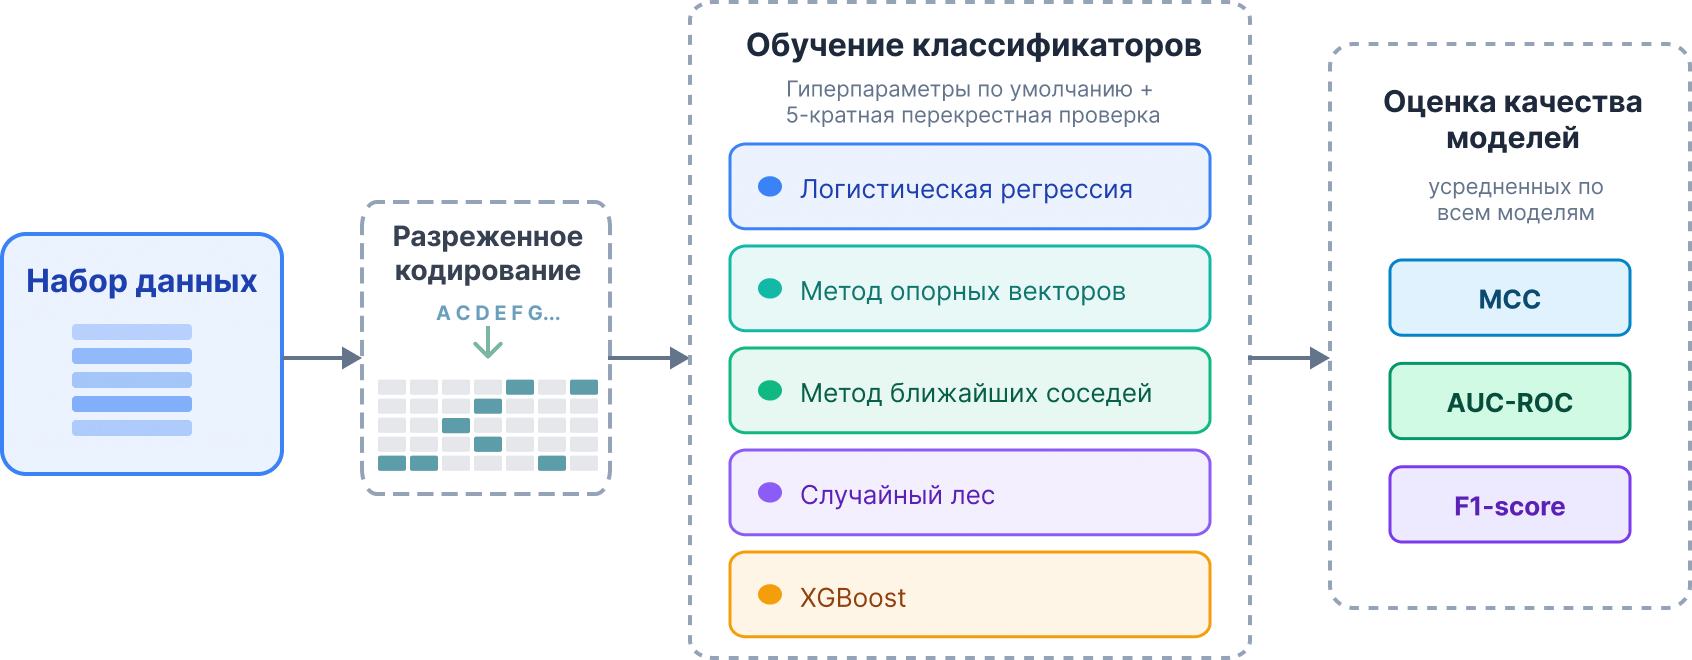
\includegraphics[width=1.0\textwidth]{images/baseline_block_flow.png}
    \caption{Схема процесса расчета базовой сложности наборов данных.}
    \label{fig:baseline_calculation}
\end{figure}

\section{Анализ характеристик сложности}

Анализ вычисленных характеристик сложности был направлен на оценку их информативности и устойчивости, а также на выявление признаков, наилучшим образом отражающих базовую сложность наборов данных.

На первом этапе все характеристики были стандартизированы путем центрирования и нормировки для обеспечения сопоставимости масштабов. 
После этого исключались признаки с низкой вариативностью, поскольку они не несут значимой информации для последующего анализа. 
В частности, были удалены такие характеристики, как минимальное расстояние Левенштейна и 
максимальное нормированное число уникальных тримеров.

\begin{figure}[h]
    \centering
    \includegraphics[width=0.8\textwidth]{images/boxplot_pivot_cv_split.png}
    \caption{Диаграммы ящиков с усами, демонстрирующие распределение коэффициента вариации для метрик сложности связанных с разнообразием последовательностей по всем контрольным наборам данных.}
    \label{fig:cv_features_sd}
\end{figure}

Далее была проведена оценка устойчивости признаков. 
Для каждого набора данных многократно формировались случайные подвыборки, составляющие 80\% исходного объема, с последующим пересчетом всех характеристик. 
На основе полученных значений вычислялся коэффициент вариации\footnote{Коэффициент вариации — это мера относительной изменчивости признака, определяемая как отношение стандартного отклонения к среднему значению. Используется для оценки устойчивости характеристик при повторных измерениях.}, отражающий относительную изменчивость признака. 
Все признаки продемонстрировали высокую стабильность, которая была ниже порогового значения в 10\%. 
Полноценные результаты этого анализа представлены на рисунках \ref{fig:cv_features_sd} и \ref{fig:cv_features_problexity} и в приложении \ref{sec:app:5:tab-data} в таблице \ref{tab:cv_features}.

\begin{figure}[h]
    \centering
    \includegraphics[width=0.8\textwidth]{images/problexity_cv.png}
    \caption{Диаграммы ящиков с усами, демонстрирующие распределение коэффициента вариации для каждой метрики сложности классификации по всем контрольным наборам данных.}
    \label{fig:cv_features_problexity}
\end{figure}


В приложении \ref{sec:app:5:tab-data} отдельно приведены распределения коэффициента вариации для энтропии классовых долей и коэффициента дисбаланса классов.
Их высокое значение среднего коэффициента вариации обусловлено прямой зависимостью значений данных показателей от объема выборки.
Также значения дополнительно смещаются при исходной несбалансированности данных.
Поэтому их исключение на основании данного критерия является некорректным.


Для оставшихся признаков анализировалась их связь с метриками качества базовых моделей. 
Корреляционный анализ на рисунке \ref{fig:correlations} демонстрирует 15 признаков, которые наиболее сильно коррелируют с базовой сложностью, однако значения всех коэффициентов не более чем умеренные. 
Наибольшую корреляцию с базовой сложностью продемонстрировали такие характеристики, как доля покрывающих данные гиперсфер, среднее число уникальных тримеров, средняя длина последовательности и энтропия Шеннона. 
Значения коэффициента Спирмена не превышали 0.57, что указывает на ограниченную объясняющую способность отдельных признаков. 
Так данные результаты подтверждают необходимость рассмотрения совокупного вклада характеристик сложности.
Абсолютные значения корреляции для всех признаков представлены в таблице \ref{tab:corr_features} в приложении \ref{sec:app:5:tab-data}.

\begin{figure}[h]
    \centering
    \includegraphics[width=0.7\textwidth]{images/feature_baseline_corr_top15.png}
    \caption{Столбчатая диаграмма коэффициентов корреляции Спирмена между признаками и базовой сложностью.}
    \label{fig:correlations}
\end{figure}

\section{Анализ информативности признаков с использованием регрессионных моделей}

После анализа устойчивости и корреляций признаков изучалась возможность аппроксимации базовой сложности наборов данных с использованием классических регрессионных моделей. 
В качестве целевых переменных рассматривались агрегированные показатели качества базовых моделей, включая MCC, F1-меру и площадь под ROC-кривой.
Для оценки использовались следующие модели:

\begin{itemize}
    \item линейная регрессия;
    \item гребневая регрессия;
    \item Lasso-регрессия;
    \item случайный лес.
\end{itemize}

Для линейной, гребневой регрессии и Lasso предварительно выполнялась стандартизация признаков путем центрирования и нормировки.

Оценка качества моделей проводилась с использованием вложенной кросс-валидации. 
Внешний цикл состоял из пятикратного разбиения данных с перемешиванием, обеспечивающего оценку обобщающей 
способности моделей.
Во внутреннем цикле выполнялся подбор подмножества из пяти признаков последовательным отбором со стратегией обратного выбора\footnote{Обратный выбор (Backward selection) — метод последовательного отбора признаков, при котором модель первоначально обучается на полном наборе признаков, после чего на каждом шаге удаляется признак, наименее улучшающий качество модели согласно выбранной функции оценки.} также с помощью пятикратной кросс-валидации.
Число признаков было выбрано как минимальное описание структурных свойств данных, которые наиболее тесно связанных с эмпирической сложностью классификации. 

В качестве основной функции качества использовался коэффициент корреляции Спирмена между истинными и предсказанными 
значениями целевой переменной. 
Использование такой метрики вместо стандартных для регрессии обусловлено тем, что базовая сложность интерпретируется 
прежде всего как относительный порядок сложности задач, а не как абсолютная непрерывная величина.

Полученные результаты для базовой сложности представлены в таблице \ref{tab:linreg_results}. 
Наилучшее качество продемонстрировала модель cлучайного леса, 
достигшая среднего коэффициента корреляции Спирмена 0.704.

\begin{table}[h]
\centering
\small
\begin{tabular}{|p{5cm}|p{4cm}|}
\hline
\textbf{Метод} & \textbf{Коэффициент корреляции Спирмена} \\ \hline

Случайный лес & 0.704 \pm 0.146 \\ \hline
Гребневая регрессия & 0.670 \pm 0.123 \\ \hline
Lasso регрессия & 0.618 \pm 0.107 \\ \hline
Линейная регрессия & 0.601 \pm 0.140 \\ \hline

\end{tabular}
\caption{Результаты предсказания базовой сложности MCC с использованием различных методов отбора признаков и регрессионных моделей.}
\label{tab:linreg_results}
\end{table}

Результаты по моделям для F1-меры и площади под ROC-кривой дополнительно представлены в приложении \ref{sec:app:5:tab-data} в таблице \ref{tab:linreg_other_results}.

Для обеспечения воспроизводимости результатов во всех процедурах использовалась фиксированная инициализация 
генератора случайных чисел ($random\_state = 42$).
Линейные модели обучались после предварительной стандартизации признаков. Для случайного леса использовалось 200 
деревьев решений и минимальный размер листа, равный двум объектам.

Лучшие модели демонстрировали умеренную корреляцию с базовой сложностью. Это указывает на то, что сложность биологических наборов данных не определяется небольшим числом доминирующих факторов и не может быть полностью описана комбинацией отдельных признаков. Вместо этого информация о сложности распределена между множеством частично коррелирующих характеристик.

Таким образом полученные результаты подтверждают наличие устойчивой статистической связи между сконструированными 
признаками и эмпирической сложностью задач.

\section{Анализ кластеров сложности}

В результате серии экспериментов, направленных на выбор оптимального и стабильного метода разбиения наборов данных на группы по признакам сложности, наилучшие результаты продемонстрировал алгоритм k-средних. 
Качество кластеризации оценивалось с использованием нескольких внутренних метрик. 
Значение коэффициента силуэта составило $0,2???$, что указывает на умеренную степень разделимости кластеров. 
Дополнительно был рассчитан коэффициент разделения кластеров, равный $0,???$, 
что показывает достаточно высокую степень разделимости кластеров в понятиях средней базовой сложности 
и разброса сложности внутри кластеров. Также коэффициент вариации размеров кластеров составил $0,???$, 
что свидетельствует об отсутствии сильного дисбаланса между группами.

Полученное разбиение характеризуется высоким коэффициентом разделения кластеров (\texttt{separation\_ratio} = 1.115), что свидетельствует о выраженных различиях между средними уровнями базовой сложности кластеров при относительно низком внутрикластерном разбросе. Значение коэффициента согласованности кластеризации между bootstrap-подвыборками составило \texttt{ARI} = 0.872, что указывает на высокую воспроизводимость выделяемой структуры данных. Дополнительно было получено высокое значение \texttt{consensus silhouette} = 0.93, подтверждающее устойчивость взаимного расположения объектов внутри кластеров. Значение показателя \texttt{PAC} составило 0.217, что свидетельствует о сравнительно низкой доле неоднозначных пар объектов и, соответственно, о стабильности границ между кластерами.

Несмотря на то что классический коэффициент силуэта для исходного пространства признаков оказался умеренным (\texttt{silhouette} = 0.263), совокупность остальных показателей демонстрирует, что выделенные группы обладают высокой устойчивостью и хорошо разделяются именно с точки зрения уровня сложности задач. Итоговое интегральное значение показателя стабильности составило \texttt{stability\_score} = 0.659, что является наилучшим результатом среди всех исследованных конфигураций кластеризации.

Для визуального анализа полученного разбиения использовался метод t-SNE\footnote{t-SNE — метод нелинейного снижения размерности, предназначенный для визуализации высокоразмерных данных. Он сохраняет локальную структуру данных, отображая близкие объекты в исходном пространстве как близкие точки в пространстве низкой размерности, что делает его удобным инструментом для анализа кластерной структуры.}. Визуализация кластеров в двумерном пространстве представлена на рисунке \ref{fig:tsne}, где наблюдается формирование отдельных групп, соответствующих различным уровням сложности. Сопоставление каждого набора данных с присвоенным кластером приведено в Приложении \ref{sec:app:2:tab-data}.

\begin{figure}[h]
    \centering
    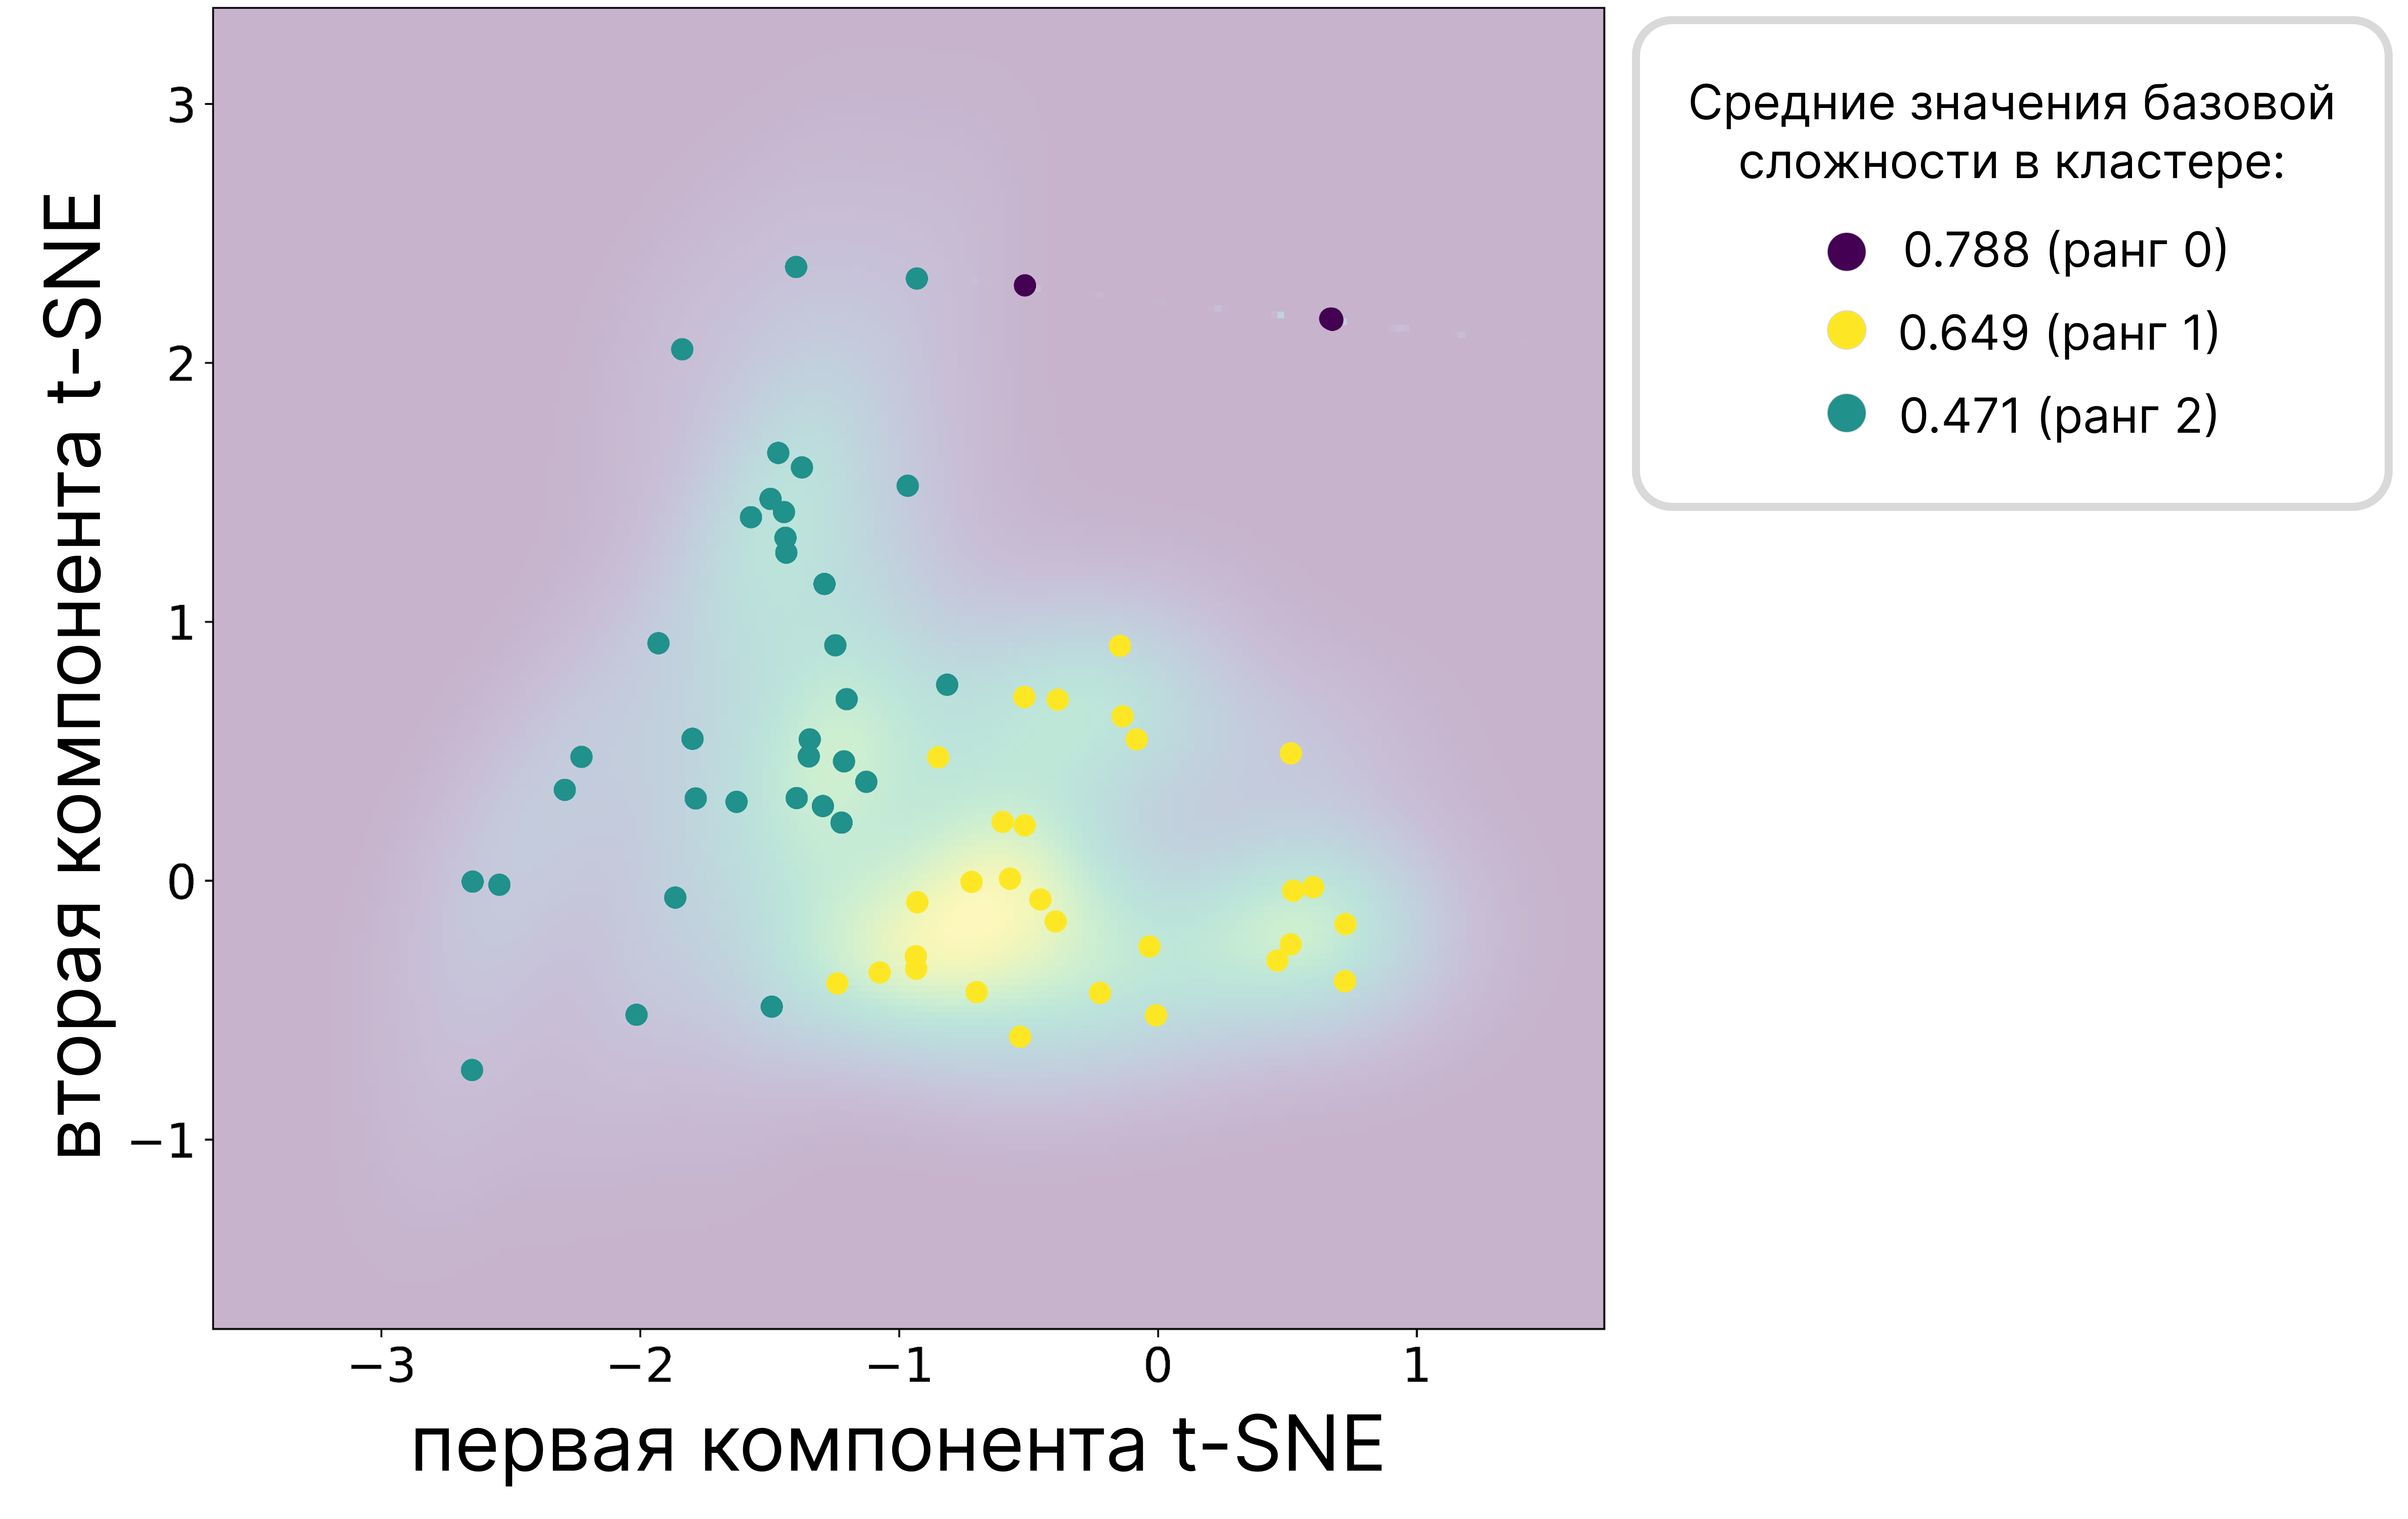
\includegraphics[width=0.8\textwidth]{images/t-SNE.png}
    \caption{Визуализация кластеров с использованием t-SNE.}
    \label{fig:tsne}
\end{figure}

Для проверки статистической значимости различий между полученными группами был применен дисперсионный анализ ANOVA\footnote{Дисперсионный анализ (ANOVA) — статистический метод, используемый для проверки гипотезы о равенстве средних значений в нескольких группах, который позволяет определить, существуют ли статистически значимые различия между кластерами по рассматриваемым признакам.}. Проведенный в приложении \ref{} в таблице \ref{} анализ показал наличие статистически значимых различий по совокупности признаков сложности, что подтверждает корректность выделенных кластеров и их интерпретацию как различных типов задач.

Профиль каждого кластера представлен на рисунке \ref{fig:radar} в виде радиальной диаграммы по десяти наиболее значимым признакам, отобранным на основе ANOVA. Наблюдаемые различия в форме и масштабе профилей свидетельствуют о том, что выделенные группы существенно отличаются друг от друга по характеристикам сложности. Это дополнительно подтверждает, что полученное разбиение является интерпретируемым и отражает реальные различия между наборами данных.

\begin{figure}[h]
    \centering
    \includegraphics[width=1.0\textwidth]{images/radar.png}
\caption{Радарные диаграммы, иллюстрирующие характеристики кластеров, упорядоченных по возрастанию средней базовой сложности. Кластер $а$ соответствует наименьшей сложности, которой соответствует ранг 0; кластер $б$ характеризуется средней сложностью и рангом 1; кластер $в$ — высокой сложностью и рангом 2.}    \label{fig:radar}
\end{figure}

Полученные кластеры были упорядочены по по возрастанию их средней сложности, что позволило перейти в дискретное пространство. 
Итоговые категории и средние значения базовой сложности каждого кластера представлены в таблице \ref{tab:clusters_rank}.

\begin{table}[h]
\centering
\small
\begin{tabular}{|p{4cm}|p{4cm}|p{3cm}|p{2cm}|}
\hline
\textbf{Категория кластера} & \textbf{Среднее значение базовой сложности} & \textbf{Колличество точек} & \textbf{Ранг} \\ \hline

Легкий & 0.788 \pm 0.053 & 7 & 0 \\ \hline
Средний & 0.649 \pm 0.116 & 29 & 1 \\ \hline
Сложный & 0.471 \pm 0.204 & 34 & 2 \\ \hline

\end{tabular}
\caption{Результаты предсказания базовой сложности MCC с использованием различных методов отбора признаков и регрессионных моделей.}
\label{tab:linreg_results}
\end{table}


Полученные результаты показывают, что использование полного набора признаков сложности совместно с агрегированным показателем MCC позволяет формировать более устойчивое и интерпретируемое разбиение пространства задач на уровни сложности. В отличие от варианта, основанного исключительно на признаках сложности, включение MCC дополнительно усиливает согласованность кластеров с эмпирически наблюдаемой трудностью классификации, что особенно важно в контексте последующего ранжирования кластеров и вычисления весов сложности при сравнении эмбеддинговых моделей.

\section{Сравнение векторных представлений передовых биологических языковых моделей}

Для демонстрации практической применимости предложенного подхода проведено тематическое исследование на примере сенсорных пептидов. В рамках собранного корпуса бенчмарков данная категория представлена тремя наборами данных. Каждый из них был отнесен к одному из ранее полученных кластеров с использованием процедуры предсказания принадлежности, основанной на рассчитанных признаках сложности. Поскольку кластеры упорядочены по возрастанию средней сложности, каждому набору данных был присвоен ранг, отражающий относительный уровень сложности задачи.

В качестве объектов сравнения рассматривались современные биологические языковые модели ESM-C, ProtBert, ProtT5 и Ankh. Для каждой модели были извлечены эмбеддинги последовательностей, после чего оценивалась их пригодность для решения задач бинарной классификации с использованием стандартных алгоритмов машинного обучения. В эксперименте использовались следующие семейства методов:
\begin{itemize}
    \item линейные модели, представленные логистической регрессией;
    \item методы опорных векторов;
    \item алгоритмы ближайших соседей;
    \item ансамблевые методы на основе решающих деревьев;
    \item методы градиентного бустинга.
\end{itemize}

Оценка качества выполнялась с применением пятикратной кросс-валидации. Для каждого набора данных и каждой языковой модели выбиралось наилучшее значение коэффициента корреляции Мэттьюса, усредненное по всем результатам пятикратной перекрестной проверки и максимизированное по всем использованным алгоритмам классификации. Таким образом, каждому набору данных сопоставлялись его ранг сложности и наилучшая достигнутая производительность для эмбеддингов каждой из рассматриваемых моделей.

На следующем этапе проводилось сравнение языковых моделей по их способности выявлять сенсорные свойства пептидов. Для этого рассчитывались два варианта агрегированной метрики качества. В первом случае использовалось простое среднее значение по всем наборам данных. Во втором случае применялось взвешенное среднее, в котором вклад каждого набора данных определялся его относительной сложностью. Веса формировались на основе рангов сложности с использованием функции softmax, что позволяло увеличить влияние более сложных задач при сохранении нормировки.

Результаты сравнения представлены в таблице \ref{tab:model_performance}. Переход к взвешенному усреднению приводит к изменению лидирующей модели. Если при использовании обычного среднего наилучший результат демонстрирует ProtT5, то с учетом сложности наборов данных преимущество переходит к Ankh, которая показывает более высокое качество на задачах повышенной сложности.

\begin{table}[h]
\centering
\small
\caption{Результаты сравнительного анализа моделей на различных наборах данных с учетом их эмпирических весов. Для каждого набора приведен ранг, отражающий относительную значимость в итоговой оценке, а также значения метрики качества для рассматриваемых моделей.}
\label{tab:model_performance}

\begin{tabular}{|p{4cm}|c|c|c|c|c|c|}
\hline
Набор данных & Ранг & Вес & ESM-C & ProtT5 & ProtBERT & Ankh \\
\hline
Набор данных 1~\cite{manavalan2018ibce} & 3 & 0.422 & 0.1736 & 0.2024 & 0.1175 & 0.1685 \\ \hline
Набор данных 2~\cite{zhao2003application} & 3 & 0.422 & 0.3666 & 0.3203 & 0.3353 & 0.3783 \\ \hline
Набор данных 3~\cite{wei2020icircda} & 2 & 0.155 & 0.8400 & 0.8621 & 0.8050 & 0.8359 \\ \hline
\end{tabular}

\end{table}

Аналогичный анализ был проведен для всех категорий бенчмарков, содержащих не менее двух наборов данных. В результате установлено, что в 35\% случаев выбор наилучшей модели изменяется при учете сложности задач. Полная сводка результатов приведена в Приложении \ref{sec:app:3:tab-data}. При этом в целом по совокупности категорий модель ProtT5 сохраняет лидерство как по обычному, так и по взвешенному среднему, что указывает на ее высокую универсальность, тогда как учет сложности позволяет выявить модели, более эффективные на трудных задачах.


\chapterconclusion

В третьей главе представлена реализация предложенного подхода и проведена его экспериментальная проверка на репрезентативном корпусе биологических данных.

Сформирован корпус из 70 наборов данных, охватывающий 19 категорий биологической активности пептидов. Для каждого набора данных вычислены характеристики сложности классификации и характеристики разнообразия последовательностей. Анализ устойчивости признаков на основе подвыборок позволил исключить нестабильные. Корреляционный анализ показал наличие статистически значимых, но умеренных зависимостей между признаками и базовой сложностью, причем наибольшую объясняющую способность продемонстрировали T1, среднее число уникальных тримеров, средняя длина последовательности и энтропия Шеннона.

По результатам сравнения методов кластеризации наилучшие показатели продемонстрировал алгоритм k-средних, сформировавший четыре кластера с коэффициентом силуэта 0,287 и коэффициентом разделения 0,720. Статистическая значимость различий между кластерами подтверждена дисперсионным анализом ANOVA, а визуализация с помощью t-SNE подтвердила наличие выраженной кластерной структуры. Полученные кластеры были ранжированы по возрастанию средней базовой сложности. Так была сформирована дискретная шкала сложности наборов данных.

Практическая применимость предложенного метода продемонстрирована при сравнении четырех современных биологических языковых моделей — ESM-C, ProtBert, ProtT5 и Ankh. Установлено, что в 35\% категорий бенчмарков переход к взвешенному усреднению приводит к изменению лидирующей модели. В частности, на примере сенсорных пептидов показано, что модель Ankh превосходит ProtT5 при учете сложности задач. В целом по совокупности категорий модель ProtT5 сохраняет лидерство, однако предложенный подход позволяет выявить модели, более эффективные на трудных задачах, что невозможно установить при стандартном усреднении.

%% Макрос для заключения. Совместим со старым стилевиком.
\startconclusionpage

В данной работе решена задача разработки метода сравнительного анализа векторных представлений биологических языковых моделей, учитывающего сложность используемых наборов данных. Предложенный подход устраняет ключевые ограничения существующих методов бенчмаркинга и обеспечивает более корректную и интерпретируемую оценку качества эмбеддингов.

В ходе выполнения работы получены следующие основные результаты:
\begin{itemize}
    \item Сформирован репрезентативный корпус из 70 наборов данных для задач бинарной классификации пептидов, охватывающий 19 категорий биологической активности. Корпус включает задачи, существенно различающиеся по объему данных, степени дисбаланса классов, разнообразию последовательностей и уровню сложности, что обеспечивает широкое покрытие пространства возможных биологических задач.
    \item Разработана система признаков, описывающих сложность наборов данных по двум взаимодополняющим аспектам: сложность классификации, отражающая геометрические и статистические свойства распределения классов, и доменная информативность, характеризующая разнообразие аминокислотных последовательностей. Введено понятие базовой эмпирической сложности, определяемой через агрегированную производительность ансамбля разнородных классификаторов на разреженном кодировании последовательностей. Показано, что данная величина устойчиво отражает структурные свойства данных и может быть аппроксимирована предложенными характеристиками.
    \item Проведен анализ устойчивости и информативности признаков сложности. По результатам бутстреп-оценки исключены нестабильные характеристики, а корреляционный анализ выявил ограниченный, но значимый набор признаков, наиболее тесно связанных с базовой сложностью. Наибольшую объясняющую способность продемонстрировали доля гиперсфер, покрывающих данные, среднее число уникальных тримеров, средняя длина последовательности и энтропия Шеннона.
    \item Разработан метод кластеризации наборов данных по уровню сложности. Сравнение нескольких алгоритмов с использованием многокритериальной системы оценки показало, что алгоритм k-средних формирует наиболее устойчивое и интерпретируемое разбиение на четыре кластера. Статистическая значимость различий между кластерами подтверждена дисперсионным анализом ANOVA, а визуализация методом t-SNE продемонстрировала наличие выраженной кластерной структуры в пространстве признаков сложности.
    \item Предложена процедура взвешенного бенчмаркинга, в которой вклад каждого набора данных в итоговую оценку языковой модели определяется рангом его кластера с применением преобразования softmax. Такое нелинейное взвешивание обеспечивает усиленный вклад сложных задач без жесткого доминирования отдельных уровней и позволяет перейти от простого усреднения метрик к более информативной агрегированной характеристике качества.
    \item Практическая применимость предложенного метода подтверждена при сравнении четырех современных биологических языковых моделей — ESM-C, ProtBert, ProtT5 и Ankh. Установлено, что в 35\% категорий бенчмарков переход к взвешенному усреднению приводит к изменению лидирующей модели. Данный результат демонстрирует, что традиционный подход систематически смещает оценки в пользу моделей, показывающих высокую производительность на простых задачах, тогда как предложенный метод позволяет выявлять модели, эффективные на задачах повышенной сложности.
\end{itemize}

Таким образом, в работе реализован переход от упрощенного усреднения метрик к структурированной и обоснованной процедуре сравнения, учитывающей неоднородность биологических данных. Предложенный подход обладает практической значимостью для выбора языковых моделей при решении прикладных задач биоинформатики, а также может быть распространен на другие типы биологических последовательностей и задачи классификации за пределами пептидной области.

Перспективными направлениями дальнейших исследований являются обобщение метода на другие биополимеры и автоматизация метода сравнения.

\printmainbibliography

%% После этой команды chapter будет генерировать приложения, нумерованные русскими буквами.
%% \startappendices из старого стилевика будет делать то же самое
\appendix

\chapter{Используемые наборы данных}\label{sec:app:1:tab-data}

\small
\begin{longtable}{
| >{\centering\arraybackslash}p{5cm}
| >{\centering\arraybackslash}p{2cm}
| >{\centering\arraybackslash}p{2.5cm}
| >{\centering\arraybackslash}p{2.5cm}
| >{\centering\arraybackslash}p{3cm} |
}
\caption{Полный перечень использованных наборов данных для задач бинарной классификации пептидов, сгруппированных по типу биологической активности. Для каждого набора указан введенный идентификатор, число положительных (класс~1) и отрицательных (класс~0) примеров, а также источник данных.}
\label{tab:datasets} \\

\hline
Тип активности & Идентификатор & Положительные примеры & Отрицательные примеры & Источник \\
\hline
\endfirsthead

\hline
Тип активности & Идентификатор & Положительные & Отрицательные & Источник \\
\hline
\endhead

\hline
\endfoot

\hline
\endlastfoot

\multirow{2}{=}{Антигипертензивные} 
& AHT-1 & 303 & 385 & \cite{nagpal2018computer} \\
\cline{2-5}
& AHT-2 & 1299 & 1299 & \cite{manavalan2019mahtpred} \\
\hline


\multirow{3}{=}{Противовоспалительные}
& INF-1 & 1451 & 2339 & \cite{raza2023aips} \\ \cline{2-5}
& INF-2 & 863 & 1261 & \cite{gupta2017prediction} \\ \cline{2-5}
& INF-3 & 420 & 629 & \cite{manavalan2018aippred} \\
\hline

\multirow{4}{=}{Антибактериальные}
& AB-1 & 148 & 847 & \cite{charoenkwan2022scmrsa} \\ \cline{2-5}
& AB-2 & 8278 & 8278 & \cite{pinacho2021alignment} \\ \cline{2-5}
& AB-3 & 246 & 246 & \cite{usmani2018prediction} \\ \cline{2-5}
& AB-4 & 246 & 246 & \cite{khatun2019efficient} \\
\hline

\multirow{6}{=}{Противоопухолевые}
& ANT-1 & 224 & 225 & \cite{tyagi2013silico} \\ \cline{2-5}
& ANT-2 & 187 & 398 & \cite{manavalan2017mlacp} \\ \cline{2-5}
& ANT-3 & 138 & 206 & \cite{chen2016iacp} \\ \cline{2-5}
& ANT-4 & 970 & 970 & \cite{charoenkwan2021improved} \\ \cline{2-5}
& ANT-5 & 861 & 861 & \cite{agrawal2021anticp} \\ \cline{2-5}
& ANT-6 & 592 & 393 & \cite{charoenkwan2020ittca} \\
\hline

\multirow{2}{=}{Антидиабетические}
& AD-1 & 236 & 236 & \cite{chen2022antidmppred} \\ \cline{2-5}
& AD-2 & 664 & 665 & \cite{charoenkwan2020idppiv} \\
\hline

\multirow{3}{=}{Противогрибковые}
& AF-1 & 1459 & 1457 & \cite{agrawal2018silico} \\ \cline{2-5}
& AF-2 & 1329 & 1384 & \cite{meher2017predicting} \\ \cline{2-5}
& AF-3 & 993 & 993 & \cite{pinacho2021alignment} \\
\hline

\multirow{3}{=}{Противопаразитарные}
& AP-1 & 138 & 677 & \cite{charoenkwan2022iamap} \\ \cline{2-5}
& AP-2 & 138 & 2069 & \cite{charoenkwan2022iamap} \\ \cline{2-5}
& AP-3 & 290 & 916 & \cite{zhang2022predapp} \\
\hline

\multirow{9}{=}{Антимикробные}
& AMP-1 & 1225 & 1354 & \cite{muller2017modlamp} \\ \cline{2-5}
& AMP-2 & 999 & 994 & \cite{su2019antimicrobial} \\ \cline{2-5}
& AMP-3 & 878 & 2405 & \cite{xiao2013iamp} \\ \cline{2-5}
& AMP-4 & 431 & 430 & \cite{lata2007analysis} \\ \cline{2-5}
& AMP-5 & 128 & 76 & \cite{porto2012cs} \\ \cline{2-5}
& AMP-6 & 115 & 116 & \cite{fernandes2012prediction} \\ \cline{2-5}
& AMP-7 & 27 & 102 & \cite{polanco2011fpga} \\ \cline{2-5}
& AMP-8 & 4134 & 4134 & \cite{cao2023designing} \\ \cline{2-5}
& AMP-9 & 6282 & 4707 & \cite{pang2022integrating} \\
\hline

\multirow{2}{=}{Противоокислительные}
& AO-1 & 1060 & 1060 & \cite{qin2023prediction} \\ \cline{2-5}
& AO-2 & 687 & 717 & \cite{olsen2020anoxpepred} \\
\hline

\multirow{12}{=}{Противовирусные}
& AV-1 & 721 & 739 & \cite{meher2017predicting} \\ \cline{2-5}
& AV-2 & 598 & 448 & \cite{thakur2012avppred} \\ \cline{2-5}
& AV-3 & 2944 & 2944 & \cite{pinacho2021alignment} \\ \cline{2-5}
& AV-4 & 43 & 112 & \cite{heider2010predicting} \\ \cline{2-5}
& AV-5 & 149 & 798 & \cite{rognvaldsson2015state} \\ \cline{2-5}
& AV-6 & 200 & 1151 & \cite{dybowski2010prediction} \\ \cline{2-5}
& AV-7 & 351 & 234 & \cite{10.1093/bioinformatics/btz493} \\ \cline{2-5}
& AV-8 & 324 & 311 & \cite{lochel2020deep} \\ \cline{2-5}
& AV-9 & 188 & 228 & \cite{lochel2020deep} \\ \cline{2-5}
& AV-10 & 249 & 403 & \cite{lochel2020deep} \\ \cline{2-5}
& AV-11 & 291 & 315 & \cite{lochel2020deep} \\ \cline{2-5}
& AV-12 & 385 & 253 & \cite{lochel2020deep} \\
\hline

\multirow{2}{=}{Вкусовые}
& TASTE-1 & 320 & 320 & \cite{charoenkwan2021bert4bitter} \\ \cline{2-5}
& TASTE-2 & 140 & 302 & \cite{charoenkwan2020iumami} \\
\hline

\multirow{1}{=}{ГЭБ-проникающие}
& BBB-1 & 119 & 119 & \cite{dai2021bbppred} \\
\hline

\multirow{7}{=}{Проникающие в клетки}
& CPP-1 & 1165 & 738 & \cite{a2010prediction} \\ \cline{2-5}
& CPP-2 & 807 & 807 & \cite{gautam2013silico} \\ \cline{2-5}
& CPP-3 & 732 & 730 & \cite{kumar2018prediction} \\ \cline{2-5}
& CPP-4 & 504 & 499 & \cite{pandey2018kelm} \\ \cline{2-5}
& CPP-5 & 462 & 462 & \cite{qiang2020cppred} \\ \cline{2-5}
& CPP-6 & 187 & 187 & \cite{manavalan2018machine} \\ \cline{2-5}
& CPP-7 & 111 & 34 & \cite{manavalan2018machine} \\
\hline

\multirow{5}{=}{Гемолитические}
& HEM-1 & 1543 & 2195 & \cite{timmons2020happenn} \\ \cline{2-5}
& HEM-2 & 522 & 582 & \cite{chaudhary2016web} \\ \cline{2-5}
& HEM-3 & 552 & 552 & \cite{plisson2020machine} \\ \cline{2-5}
& HEM-4 & 552 & 462 & \cite{plisson2020machine} \\ \cline{2-5}
& HEM-5 & 884 & 738 & \cite{plisson2020machine} \\
\hline

\multirow{1}{*}{Иммуносупрессивные}
& IMM-1 & 394 & 848 & \cite{nagpal2017computer} \\
\hline

\multirow{3}{=}{Сенсорные}
& SEN-1 & 1110 & 1408 & \cite{manavalan2018ibce} \\ \cline{2-5}
& SEN-2 & 36 & 167 & \cite{zhao2003application} \\ \cline{2-5}
& SEN-3 & 218 & 214 & \cite{wei2020icircda} \\
\hline

\multirow{2}{=}{Нейропептиды}
& NP-1 & 2425 & 2425 & \cite{chen2022neuropred} \\ \cline{2-5}
& NP-2 & 875 & 875 & \cite{agrawal2019neuropipred} \\
\hline

\multirow{1}{=}{Провоспалительные}
& PINF-1 & 833 & 2395 & \cite{manavalan2018pip} \\
\hline

\multirow{2}{=}{Токсичные}
& TOX-1 & 2138 & 5375 & \cite{gao2025plptp} \\ \cline{2-5}
& TOX-2 & 1932 & 1932 & \cite{wei2021atse} \\
\hline

\end{longtable}

\chapter{Результаты оценки сложности наборов данных.}\label{sec:app:4:tab-data}

\small
\begin{longtable}{
| >{\centering\arraybackslash}p{3cm}
| >{\centering\arraybackslash}p{4cm}
| >{\centering\arraybackslash}p{4cm}
| >{\centering\arraybackslash}p{4cm} |
}

\caption{Результаты оценки качества базовых моделей на наборах данных пептидов, используемые для анализа их базовой сложности, по метрикам MCC, F1 и AUC-ROC (стратифицированная 5-fold кросс-валидация, среднее значение и стандартное отклонение).}
\label{tab:metrics_comparison} \\

\hline
Идентификатор набора данных 
& Средний MCC 
& Средний F1 
& Средний AUC\_ROC \\
\hline
\endfirsthead

\hline
Идентификатор набора данных 
& Средний MCC 
& Средний F1 
& Средний AUC\_ROC \\
\hline
\endhead

\hline
\endfoot

\hline
\endlastfoot

AB-1 & 0.577 $\pm$ 0.098 & 0.586 $\pm$ 0.1 & 0.723 $\pm$ 0.052 \\ \hline
AB-2 & 0.757 $\pm$ 0.136 & 0.88 $\pm$ 0.057 & 0.876 $\pm$ 0.072 \\ \hline
AB-3 & 0.545 $\pm$ 0.033 & 0.742 $\pm$ 0.043 & 0.765 $\pm$ 0.02 \\ \hline
AB-4 & 0.426 $\pm$ 0.058 & 0.676 $\pm$ 0.058 & 0.706 $\pm$ 0.031 \\ \hline
AD-1 & 0.229 $\pm$ 0.067 & 0.617 $\pm$ 0.028 & 0.614 $\pm$ 0.034 \\ \hline
AD-2 & 0.584 $\pm$ 0.269 & 0.818 $\pm$ 0.082 & 0.784 $\pm$ 0.15 \\ \hline
AF-1 & 0.606 $\pm$ 0.193 & 0.812 $\pm$ 0.076 & 0.801 $\pm$ 0.101 \\ \hline
AF-2 & 0.686 $\pm$ 0.127 & 0.839 $\pm$ 0.057 & 0.842 $\pm$ 0.064 \\ \hline
AF-3 & 0.712 $\pm$ 0.271 & 0.857 $\pm$ 0.129 & 0.855 $\pm$ 0.136 \\ \hline
AHT-1 & 0.792 $\pm$ 0.077 & 0.885 $\pm$ 0.039 & 0.896 $\pm$ 0.037 \\ \hline
AHT-2 & 0.542 $\pm$ 0.117 & 0.777 $\pm$ 0.042 & 0.768 $\pm$ 0.063 \\ \hline
AMP-1 & 0.809 $\pm$ 0.05 & 0.902 $\pm$ 0.025 & 0.905 $\pm$ 0.025 \\ \hline
AMP-2 & 0.7 $\pm$ 0.126 & 0.85 $\pm$ 0.053 & 0.848 $\pm$ 0.065 \\ \hline
AMP-3 & 0.593 $\pm$ 0.309 & 0.726 $\pm$ 0.169 & 0.794 $\pm$ 0.159 \\ \hline
AMP-4 & 0.793 $\pm$ 0.076 & 0.896 $\pm$ 0.033 & 0.892 $\pm$ 0.045 \\ \hline
AMP-5 & 0.669 $\pm$ 0.376 & 0.907 $\pm$ 0.077 & 0.824 $\pm$ 0.183 \\ \hline
AMP-6 & 0.445 $\pm$ 0.125 & 0.737 $\pm$ 0.047 & 0.716 $\pm$ 0.068 \\ \hline
AMP-7 & 0.79 $\pm$ 0.062 & 0.806 $\pm$ 0.05 & 0.876 $\pm$ 0.018 \\ \hline
AMP-8 & 0.589 $\pm$ 0.08 & 0.79 $\pm$ 0.025 & 0.792 $\pm$ 0.041 \\ \hline
AMP-9 & 0.699 $\pm$ 0.391 & 0.901 $\pm$ 0.097 & 0.851 $\pm$ 0.197 \\ \hline
ANT-1 & 0.579 $\pm$ 0.101 & 0.765 $\pm$ 0.08 & 0.784 $\pm$ 0.054 \\ \hline
ANT-2 & 0.501 $\pm$ 0.101 & 0.645 $\pm$ 0.039 & 0.735 $\pm$ 0.034 \\ \hline
ANT-3 & 0.633 $\pm$ 0.185 & 0.775 $\pm$ 0.081 & 0.801 $\pm$ 0.091 \\ \hline
ANT-4 & 0.711 $\pm$ 0.115 & 0.853 $\pm$ 0.05 & 0.854 $\pm$ 0.058 \\ \hline
ANT-5 & 0.446 $\pm$ 0.051 & 0.726 $\pm$ 0.011 & 0.721 $\pm$ 0.029 \\ \hline
ANT-6 & 0.291 $\pm$ 0.122 & 0.75 $\pm$ 0.046 & 0.628 $\pm$ 0.047 \\ \hline
AO-1 & 0.793 $\pm$ 0.08 & 0.891 $\pm$ 0.046 & 0.895 $\pm$ 0.041 \\ \hline
AO-2 & 0.457 $\pm$ 0.053 & 0.706 $\pm$ 0.037 & 0.726 $\pm$ 0.027 \\ \hline
AP-1 & 0.626 $\pm$ 0.351 & 0.703 $\pm$ 0.232 & 0.785 $\pm$ 0.16 \\ \hline
AP-2 & 0.601 $\pm$ 0.261 & 0.596 $\pm$ 0.248 & 0.755 $\pm$ 0.075 \\ \hline
AP-3 & 0.425 $\pm$ 0.191 & 0.559 $\pm$ 0.093 & 0.687 $\pm$ 0.096 \\ \hline
AV-1 & 0.492 $\pm$ 0.104 & 0.74 $\pm$ 0.041 & 0.745 $\pm$ 0.052 \\ \hline
AV-10 & 0.795 $\pm$ 0.079 & 0.874 $\pm$ 0.047 & 0.901 $\pm$ 0.037 \\ \hline
AV-11 & 0.845 $\pm$ 0.082 & 0.921 $\pm$ 0.04 & 0.92 $\pm$ 0.045 \\ \hline
AV-12 & 0.755 $\pm$ 0.052 & 0.904 $\pm$ 0.017 & 0.873 $\pm$ 0.034 \\ \hline
AV-2 & 0.453 $\pm$ 0.108 & 0.752 $\pm$ 0.077 & 0.726 $\pm$ 0.054 \\ \hline
AV-3 & 0.497 $\pm$ 0.097 & 0.734 $\pm$ 0.03 & 0.745 $\pm$ 0.046 \\ \hline
AV-4 & 0.644 $\pm$ 0.055 & 0.718 $\pm$ 0.059 & 0.806 $\pm$ 0.042 \\ \hline
AV-5 & 0.494 $\pm$ 0.142 & 0.487 $\pm$ 0.185 & 0.684 $\pm$ 0.101 \\ \hline
AV-6 & 0.832 $\pm$ 0.04 & 0.849 $\pm$ 0.042 & 0.889 $\pm$ 0.036 \\ \hline
AV-7 & 0.688 $\pm$ 0.063 & 0.878 $\pm$ 0.019 & 0.84 $\pm$ 0.038 \\ \hline
AV-8 & 0.811 $\pm$ 0.061 & 0.909 $\pm$ 0.027 & 0.903 $\pm$ 0.035 \\ \hline
AV-9 & 0.789 $\pm$ 0.059 & 0.884 $\pm$ 0.028 & 0.892 $\pm$ 0.03 \\ \hline
BBB-1 & 0.382 $\pm$ 0.169 & 0.718 $\pm$ 0.03 & 0.687 $\pm$ 0.091 \\ \hline
CPP-1 & 0.599 $\pm$ 0.184 & 0.757 $\pm$ 0.081 & 0.787 $\pm$ 0.096 \\ \hline
CPP-2 & 0.664 $\pm$ 0.129 & 0.833 $\pm$ 0.051 & 0.83 $\pm$ 0.067 \\ \hline
CPP-3 & 0.784 $\pm$ 0.043 & 0.89 $\pm$ 0.022 & 0.892 $\pm$ 0.021 \\ \hline
CPP-4 & 0.605 $\pm$ 0.068 & 0.811 $\pm$ 0.027 & 0.8 $\pm$ 0.037 \\ \hline
CPP-5 & 0.646 $\pm$ 0.079 & 0.821 $\pm$ 0.043 & 0.821 $\pm$ 0.038 \\ \hline
CPP-6 & 0.204 $\pm$ 0.027 & 0.603 $\pm$ 0.018 & 0.601 $\pm$ 0.013 \\ \hline
CPP-7 & -0.016 $\pm$ 0.107 & 0.843 $\pm$ 0.014 & 0.501 $\pm$ 0.043 \\ \hline
HEM-1 & 0.573 $\pm$ 0.041 & 0.74 $\pm$ 0.023 & 0.782 $\pm$ 0.02 \\ \hline
HEM-2 & 0.8 $\pm$ 0.054 & 0.895 $\pm$ 0.027 & 0.9 $\pm$ 0.027 \\ \hline
HEM-3 & 0.86 $\pm$ 0.066 & 0.929 $\pm$ 0.031 & 0.929 $\pm$ 0.034 \\ \hline
HEM-4 & 0.498 $\pm$ 0.045 & 0.768 $\pm$ 0.031 & 0.748 $\pm$ 0.022 \\ \hline
HEM-5 & 0.507 $\pm$ 0.044 & 0.771 $\pm$ 0.037 & 0.752 $\pm$ 0.021 \\ \hline
IMM-1 & 0.315 $\pm$ 0.087 & 0.472 $\pm$ 0.037 & 0.631 $\pm$ 0.027 \\ \hline
INF-1 & 0.23 $\pm$ 0.089 & 0.486 $\pm$ 0.039 & 0.606 $\pm$ 0.04 \\ \hline
INF-2 & 0.236 $\pm$ 0.069 & 0.519 $\pm$ 0.026 & 0.611 $\pm$ 0.031 \\ \hline
INF-3 & 0.184 $\pm$ 0.088 & 0.451 $\pm$ 0.056 & 0.583 $\pm$ 0.039 \\ \hline
NP-1 & 0.627 $\pm$ 0.104 & 0.82 $\pm$ 0.038 & 0.809 $\pm$ 0.06 \\ \hline
NP-2 & 0.683 $\pm$ 0.075 & 0.825 $\pm$ 0.047 & 0.837 $\pm$ 0.039 \\ \hline
PINF-1 & 0.271 $\pm$ 0.122 & 0.37 $\pm$ 0.089 & 0.601 $\pm$ 0.047 \\ \hline
SEN-1 & 0.168 $\pm$ 0.072 & 0.499 $\pm$ 0.033 & 0.581 $\pm$ 0.034 \\ \hline
SEN-2 & 0.474 $\pm$ 0.042 & 0.521 $\pm$ 0.065 & 0.709 $\pm$ 0.057 \\ \hline
SEN-3 & 0.672 $\pm$ 0.216 & 0.85 $\pm$ 0.082 & 0.821 $\pm$ 0.137 \\ \hline
TASTE-1 & 0.559 $\pm$ 0.076 & 0.783 $\pm$ 0.026 & 0.776 $\pm$ 0.042 \\ \hline
TASTE-2 & 0.569 $\pm$ 0.071 & 0.683 $\pm$ 0.058 & 0.767 $\pm$ 0.039 \\ \hline
TOX-1 & 0.767 $\pm$ 0.07 & 0.825 $\pm$ 0.062 & 0.869 $\pm$ 0.047 \\ \hline
TOX-2 & 0.801 $\pm$ 0.052 & 0.901 $\pm$ 0.025 & 0.9 $\pm$ 0.026 \\ \hline

\end{longtable}

\chapter{Анализ признаков.}\label{sec:app:5:tab-data}


\begin{longtable}{
| >{\centering\arraybackslash}p{3.2cm}
| >{\centering\arraybackslash}p{3.5cm}
| >{\centering\arraybackslash}p{3.5cm}
| >{\centering\arraybackslash}p{3.2cm} |
}

\caption{Результаты анализа устойчивости признаков на основе подвыборок. Для каждого признака приведены среднее значение, стандартное отклонение и коэффициент вариации (CV), характеризующий относительную изменчивость.}
\label{tab:cv_features} \\

\hline
Признак & Среднее значение признака & Стандартное отклонение & Коэффициент вариации (CV) \\
\hline
\endfirsthead

\hline
Признак & Среднее значение признака & Стандартное отклонение & Коэффициент вариации (CV) \\
\hline
\endhead

\hline
\endfoot

\hline
\endlastfoot

C1 & 0.068 & 0.005 & 1.664  \\ \hline
C2 & 0.126 & 0.009 & 0.953  \\ \hline
LSC & 0.985 & 0.002 & 0.002  \\ \hline
T1 & 0.857 & 0.012 & 0.015  \\ \hline
clsCoef & 0.598 & 0.02 & 0.051  \\ \hline
density & 0.934 & 0.007 & 0.008  \\ \hline
LenEntr & 2.01 & 0.026 & 0.014  \\ \hline
LenMax & 67.24 & 1.609 & 0.023  \\ \hline
LenMean & 30.465 & 0.15 & 0.006  \\ \hline
LenMed & 28.66 & 0.203 & 0.01  \\ \hline
LenMin & 15.702 & 0.105 & 0.028  \\ \hline
LenStd & 9.629 & 0.141 & 0.017  \\ \hline
LevEntr & 1.781 & 0.03 & 0.019  \\ \hline
LevMax & 59.729 & 1.736 & 0.028  \\ \hline
LevMean & 23.205 & 0.175 & 0.008  \\ \hline
LevMed & 22.411 & 0.293 & 0.013  \\ \hline
LevStd & 8.682 & 0.166 & 0.02  \\ \hline
NTriEntr & 0.854 & 0.057 & 0.092  \\ \hline
NTriMean & 0.954 & 0.002 & 0.002  \\ \hline
NTriMed & 0.99 & 0.0 & 0.0  \\ \hline
NTriMin & 0.307 & 0.032 & 0.25  \\ \hline
NTriStd & 0.096 & 0.003 & 0.048  \\ \hline
ShEntrEntr & 2.596 & 0.028 & 0.012  \\ \hline
ShEntrMax & 3.979 & 0.018 & 0.005  \\ \hline
ShEntrMean & 3.061 & 0.008 & 0.003  \\ \hline
ShEntrMed & 3.13 & 0.009 & 0.003  \\ \hline
ShEntrMin & 1.036 & 0.089 & 0.539  \\ \hline
ShEntrStd & 0.472 & 0.007 & 0.015  \\ \hline
TriEntr & 2.132 & 0.028 & 0.02  \\ \hline
TriMax & 63.79 & 1.646 & 0.025  \\ \hline
TriMean & 27.298 & 0.144 & 0.008  \\ \hline
TriMed & 25.751 & 0.231 & 0.017  \\ \hline
TriMin & 11.106 & 0.359 & 0.223  \\ \hline
TriStd & 9.415 & 0.136 & 0.022  \\ \hline

\end{longtable}

\begin{figure}[h]
    \centering
    \includegraphics[width=0.8\textwidth]{images/violinplot_C1.png}
    \caption{Скрипичный график распределения коэффициента вариации энтропии классовых долей.}
    \label{fig:vp_c1_cv}
\end{figure}

\begin{figure}[h]
    \centering
    \includegraphics[width=0.8\textwidth]{images/violinplot_C2.png}
    \caption{Скрипичный график распределения коэффициента вариации коэффициента дисбаланса классов.}
    \label{fig:vp_c2_cv}
\end{figure}

\begin{longtable}{
| >{\centering\arraybackslash}p{3.2cm}
| >{\centering\arraybackslash}p{3.5cm}
| >{\centering\arraybackslash}p{3.5cm}
| >{\centering\arraybackslash}p{3.2cm} |
}

\caption{Значения коэффициентов корреляции Спирмена между признаками и производительностью моделей базовой линии. Все значения производительности были взяты как среднее значение метрики на пятикратной кросс-валидации.}
\label{tab:corr_features} \\

\hline
Признак & MCC & AUC-ROC & F1-мера \\
\hline
\endfirsthead

\hline
Признак & MCC & AUC-ROC & F1-мера \\
\hline
\endhead

\hline
\endfoot

\hline
\endlastfoot

C1 & -0.13 & -0.217 & -0.345  \\ \hline
C2 & -0.115 & -0.2 & -0.331  \\ \hline
LSC & -0.336 & -0.309 & -0.353  \\ \hline
T1 & -0.577 & -0.596 & -0.618  \\ \hline
density & -0.305 & -0.331 & -0.356  \\ \hline
clsCoef & -0.378 & -0.415 & -0.451  \\ \hline
LevEntr & 0.305 & 0.313 & 0.273  \\ \hline
LevMean & 0.161 & 0.157 & 0.149  \\ \hline
LevStd & 0.203 & 0.221 & 0.25  \\ \hline
LevMed & 0.167 & 0.161 & 0.147  \\ \hline
LevMax & 0.089 & 0.109 & 0.152  \\ \hline
LenEntr & 0.119 & 0.149 & 0.145  \\ \hline
LenMean & 0.541 & 0.524 & 0.476  \\ \hline
LenStd & 0.074 & 0.084 & 0.093  \\ \hline
LenMed & 0.497 & 0.479 & 0.433  \\ \hline
LenMin & 0.186 & 0.168 & 0.154  \\ \hline
LenMax & 0.324 & 0.349 & 0.405  \\ \hline
ShEntrEntr & 0.122 & 0.133 & 0.085  \\ \hline
ShEntrMean & 0.429 & 0.399 & 0.298  \\ \hline
ShEntrStd & -0.118 & -0.085 & -0.039  \\ \hline
ShEntrMed & 0.448 & 0.42 & 0.323  \\ \hline
ShEntrMin & 0.249 & 0.227 & 0.182  \\ \hline
ShEntrMax & 0.423 & 0.419 & 0.384  \\ \hline
TriEntr & 0.149 & 0.183 & 0.183  \\ \hline
TriMean & 0.542 & 0.523 & 0.465  \\ \hline
TriStd & 0.115 & 0.125 & 0.13  \\ \hline
TriMed & 0.52 & 0.499 & 0.438  \\ \hline
TriMin & 0.244 & 0.221 & 0.19  \\ \hline
TriMax & 0.362 & 0.382 & 0.405  \\ \hline
NTriEntr & 0.21 & 0.236 & 0.3  \\ \hline
NTriMean & -0.145 & -0.185 & -0.255  \\ \hline
NTriStd & -0.126 & -0.096 & -0.061  \\ \hline
NTriMed & -0.286 & -0.303 & -0.333  \\ \hline
NTriMin & 0.109 & 0.085 & 0.092  \\ \hline

\end{longtable}

\begin{table}[h]
\centering
\small
\begin{tabular}{|p{5cm}|p{4cm}|p{4cm}|}
\hline
\textbf{Метод} & \textbf{Коэффициенткорреляции Спирмена для F1-меры} & \textbf{Коэффициенткорреляции Спирмена для ROC-AUC} \\ \hline

Случайный лес & 0.647 \pm 0.212 & 0.636 \pm 0.171 \\ \hline
Гребневая регрессия & 0.575 \pm 0.300 & 0.645 \pm 0.132 \\ \hline
Lasso регрессия & 0.636 \pm 0.255 & 0.627 \pm 0.135 \\ \hline
Линейная регрессия & 0.558 \pm 0.216 & 0.573 \pm 0.152 \\ \hline

\end{tabular}
\caption{Результаты предсказания качества моделей через F1-меру и ROC-AUC с использованием различных регрессионных моделей.}
\label{tab:linreg_other_results}
\end{table}

\chapter{Результаты оценки сложности наборов данных.}\label{sec:app:2:tab-data}

\small
\begin{longtable}{
| >{\centering\arraybackslash}p{7cm}
| >{\centering\arraybackslash}p{7cm}|
}

\caption{Эмпирическая категоризация сложности наборов данных и соответствующее ей числовое представление. Для каждого набора данных указан уровень сложности (очень низкая, низкая, средняя, высокая), определенный на основе экспертной оценки, а также числовой коэффициент, используемый при расчете взвешенных метрик качества моделей.}
\label{tab:dataset_difficulty} \\

\hline
Идентификатор набора данных & Категория сложности набора данных \\
\hline
\endfirsthead

\hline
Идентификатор набора данных & Категория сложности набора данных \\
\hline
\endhead

\hline
\endfoot

\hline
\endlastfoot

TASTE-2 & сложный\\ \hline
ANT-6 & сложный\\ \hline
TOX-1 & средний\\ \hline
TOX-2 & средний\\ \hline
SEN-2 & сложный\\ \hline
SEN-3 & средний\\ \hline
PINF-1 & сложный\\ \hline
NP-1 & средний\\ \hline
NP-2 & средний\\ \hline
IMM-1 & сложный\\ \hline
AV-6 & легкий\\ \hline
AV-12 & легкий\\ \hline
AV-11 & легкий\\ \hline
AV-5 & сложный\\ \hline
AV-10 & легкий\\ \hline
AV-9 & легкий\\ \hline
AV-8 & легкий\\ \hline
AV-4 & сложный\\ \hline
AV-7 & легкий\\ \hline
HEM-2 & средний\\ \hline
CPP-7 & сложный\\ \hline
CPP-6 & сложный\\ \hline
CPP-1 & сложный\\ \hline
CPP-4 & сложный\\ \hline
CPP-5 & сложный\\ \hline
CPP-3 & сложный\\ \hline
CPP-2 & сложный\\ \hline
BBB-1 & сложный\\ \hline
TASTE-1 & сложный\\ \hline
SEN-1 & сложный\\ \hline
AV-2 & средний\\ \hline
AV-1 & средний\\ \hline
AB-4 & сложный\\ \hline
AB-3 & сложный\\ \hline
AV-3 & средний\\ \hline
AP-3 & средний\\ \hline
AO-2 & сложный\\ \hline
AO-1 & сложный\\ \hline
AMP-9 & средний\\ \hline
AMP-8 & сложный\\ \hline
AP-2 & средний\\ \hline
AP-1 & средний\\ \hline
AF-3 & средний\\ \hline
AD-1 & сложный\\ \hline
ANT-5 & сложный\\ \hline
ANT-4 & средний\\ \hline
AB-2 & средний\\ \hline
AB-1 & средний\\ \hline
INF-1 & сложный\\ \hline
AMP-1 & средний\\ \hline
AMP-3 & средний\\ \hline
AMP-7 & средний\\ \hline
AMP-6 & сложный\\ \hline
AMP-5 & средний\\ \hline
AMP-2 & средний\\ \hline
AMP-4 & сложный\\ \hline
INF-2 & сложный\\ \hline
INF-3 & сложный\\ \hline
AF-1 & средний\\ \hline
AF-2 & средний\\ \hline
ANT-2 & сложный\\ \hline
ANT-3 & средний\\ \hline
ANT-1 & средний\\ \hline
AHT-1 & сложный\\ \hline
AHT-2 & сложный\\ \hline
HEM-1 & сложный\\ \hline
HEM-5 & средний\\ \hline
HEM-4 & средний\\ \hline
HEM-3 & средний\\ \hline
AD-2 & сложный\\ \hline

\end{longtable}


\chapter{Результаты сравнительного анализа моделей по категориям биологической активности}\label{sec:app:3:tab-data}

\begin{table}[h]
\centering
\small
\caption{Сравнение лучших моделей кодирования пептидных последовательностей по типам биологической активности. Представлены модели, демонстрирующие наилучшее среднее качество и взвешенное среднее качество по соответствующим наборам задач.}
\label{tab:best_models_by_type}

\begin{tabular}{|p{4.5cm}|p{5cm}|p{5cm}|}
\hline
Тип биологической активности & Лучшая модель (среднее качество) & Лучшая модель (взвешенное качество) \\
\hline
Противовирусные & Ankh & ESM-C \\ \hline
Антимикробные & ProtT5 & ProtT5 \\ \hline
Проникающие в клетки & ProtT5 & ESM-C \\ \hline
Противоопухолевые & ProtT5 & ProtT5 \\ \hline
Гемолитические & Ankh & Ankh \\ \hline
Антибактериальные & ProtT5 & ESM-C \\ \hline
Противогрибковые & Ankh & Ankh \\ \hline
Противопаразитарные & ProtT5 & ProtT5 \\ \hline
Сенсорные & ProtT5 & Ankh \\ \hline
Противовоспалительные & ProtT5 & ProtT5 \\ \hline
Антигипертензивные & Ankh & Ankh \\ \hline
Антидиабетические & ESM-C & ESM-C \\ \hline
Вкусовые & ProtT5 & ProtT5 \\ \hline
Противоокислительные & ProtT5 & ProtT5 \\ \hline
Нейропептиды & ESM-C & Ankh \\ \hline
Токсичные & ProtT5 & ProtT5 \\ \hline
Другие & ESM-C & ProtT5 \\ \hline

\end{tabular}

\end{table}

\end{document}